% LaTeX source for book ``代数学方法'' in Chinese
% Copyright 2018  李文威 (Wen-Wei Li).
% Permission is granted to copy, distribute and/or modify this
% document under the terms of the Creative Commons
% Attribution 4.0 International (CC BY 4.0)
% http://creativecommons.org/licenses/by/4.0/

% To be included
\chapter{幺半范畴}\label{sec:monoidal-cat}
幺半范畴原名``带乘法的范畴'', 它是带有类似于乘法的运算 $\otimes$ 和幺对象 $\munit$ 的范畴结构, 并且在精确到自然同构的意义下具有结合性与幺元性质等约束. 幺半范畴在数学物理和几何等领域中有出色应用. 除此之外, 它既是表述其它范畴论构造的方便语言, 更是进一步熟悉范畴论技巧的极佳机会, 这是本书决定尽早引入幺半范畴概念的原因. 尽管其定义对初学者可能稍显复杂, 却有两个极具体的例子:
\begin{enumerate}
	\item 向量空间的张量积 $\otimes$, 或者更广泛地说, 交换环上的模的张量积, 这在 \S\ref{sec:module-tensor-prod} 将有仔细的辨析;
	\item 拓扑学中的直观实例, 将在 \S\ref{sec:braiding} 探讨的辫范畴 $\cate{Braid}$ 就是一个例子.
\end{enumerate}

充实范畴是数学工作者日用而不知的概念, 我们将在 \S\ref{sec:enriched-cat} 道个明白, 随后在 \S\ref{sec:2-cat} 解释 $2$-范畴的基本想法. 两者都基于幺半范畴的语言.

关于幺半范畴的进一步理论与应用, 可参阅 \cite{EGNO15}.

\begin{wenxintishi}
	幺半范畴的原型是模的张量积 $\otimes$. 对此我们只会在 \S\ref{sec:enriched-cat} 用到最简单的 $\Z$-模情形, 亦即交换群的张量积. 倘若读者对交换环上的模及其张量积具备基本知识, 或者至少了解向量空间的情形, 将有助于理解本章的许多例子; 如果读者还不熟悉相关的代数或几何背景, 可考虑暂时略过. 本章后半部的 $\cate{Ab}$-范畴, 加性范畴和双积之后将派上用场, 不必动用幺半范畴就可以理解这些概念.

	由于这部分的定义和证明稍长, 初次接触时宜先以体会概略想法与实例为初步目标; 另一种办法则是待后续章节如 \S\ref{sec:modules} 碰上时再回头研读. 无须强记相关概念.

	部分文献中改用所谓张量范畴或 $\otimes$-范畴的概念, 一些定义也有细微出入, 读者宜多留意. \index{zhangliangfanchou@张量范畴 (tensor category)}
\end{wenxintishi}

\section{基本定义}\label{sec:monoidal-cat-def}
本节不涉及集合论问题, 以下定义取自 \cite[\S 2.1]{EGNO15}.

\begin{definition}\label{def:monoidal-cat} \index{yaobanfanchou@幺半范畴 (monoidal category)}\index[sym1]{1otimes@$\otimes$}
	\emph{幺半范畴}意指一组资料 $(\mathcal{V}, \otimes, a, \munit, \iota)$, 其中
	\begin{enumerate}[(i)]
		\item $\mathcal{V}$ 是一个范畴;
		\item $\otimes: \mathcal{V} \times \mathcal{V} \to \mathcal{V}$ 是二元函子, 其在对象和态射集上定义的映射分别记为 $(X,Y) \mapsto X \otimes Y$ 和 $(f,g) \mapsto f \otimes g$;
		\item $a$ 是函子范畴 $\text{Fct}(\mathcal{V} \times \mathcal{V} \times \mathcal{V}, \mathcal{V})$ 中的同构
			\[ a: ((\cdot \otimes \cdot) \otimes \cdot) \rightiso (\cdot \otimes (\cdot \otimes \cdot)), \]
			使得对所有对象 $X,Y,Z,W$, 下图交换.
			\begin{center}\begin{tikzpicture}[commutative diagrams/every diagram]
				\node (P0) at (90:2.3cm) {$((X \otimes Y) \otimes Z) \otimes W$};
				\node (P1) at (90+72:2cm) {$(X \otimes (Y \otimes Z)) \otimes W$} ;
				\node (P2) at (90+2*72:2cm) {\makebox[5ex][r]{$X \otimes ((Y \otimes Z) \otimes W)$}};
				\node (P3) at (90+3*72:2cm) {\makebox[5ex][l]{$X \otimes (Y \otimes (Z \otimes W))$}};
				\node (P4) at (90+4*72:2cm) {$(X \otimes Y) \otimes (Z \otimes W)$};

				\path[commutative diagrams/.cd, every arrow, every label]
				(P0) edge node[swap] {$a(X,Y,Z) \otimes \identity_W$} (P1)
				(P1) edge node[swap] {$a(X, Y \otimes Z, W)$} (P2)
				(P2) edge node[swap, inner sep=1em] {$\identity_X \otimes a(Y,Z,W)$} (P3)
				(P4) edge node {$a(X, Y, Z \otimes W)$} (P3)
				(P0) edge node {$a(X \otimes Y, Z, W)$} (P4);
			\end{tikzpicture}\end{center}
		\item 对象 $\munit \in \Obj(\mathcal{V})$ 称为幺元, 相应的函子 $\munit \otimes -$ 和 $- \otimes \munit$ 须给出范畴 $\mathcal{V}$ 到自身的等价;\index{duixiang!幺对象 (unit object)}
		\item $\iota: \munit \otimes \munit \rightiso \munit$.
	\end{enumerate}
\end{definition}

这里的 $a$ 又称\emph{结合约束}\index{jieheyueshu}. 我们习惯将 $\otimes$ 想成某种二元运算, 现实中 $\otimes$ 鲜少具备严格结合律 $(X \otimes Y) \otimes Z = X \otimes (Y \otimes Z)$, 因此退而求其次, 将结合律的等式改成一族给定的``约束'' $a(X, Y, Z): (X \otimes Y) \otimes Z \rightiso X \otimes (Y \otimes Z)$, 使得 $a$ 对各变元皆自然. 由于结合约束可以反复套用, $a$ 还应具备 (iii) 的相容条件. 此交换图表称为 MacLane 的五角形公理\index{MacLane 五角形公理}, 画法是以 $X,Y,Z,W$ 循序相乘的所有可能方式作为图的顶点; 能应用一次结合约束 $a$ 相连的以边连接. 同理, 幺元 $\munit$ 满足的并非严格等式 $\munit \otimes \munit = \munit$, 而是自然同构 $\iota$.

这也再次见证了范畴论中严格等同与同构概念的差别, 见注记 \ref{rem:strict-or-not}.

\begin{definition}\label{def:monoidal-constraints}
	给定幺半范畴 $(\mathcal{V}, \otimes, a, \munit, \iota)$ 和对象 $X$, 由于 $\munit \otimes -$ 和 $- \otimes \munit$ 给出范畴等价 $\mathcal{V} \to \mathcal{V}$, 我们可以
	\begin{compactitem}
		\item 唯一地定义 $ \lambda_X: \munit \otimes X \rightiso X$ 使得
			\[ \identity_{\munit} \otimes \lambda_X = \left[ \munit \otimes (\munit \otimes X) \xrightarrow{ a(\munit, \munit, X)^{-1} } (\munit \otimes \munit) \otimes X \xrightarrow{\iota \otimes \identity_X} \munit \otimes X \right] ; \]
		\item 同理可唯一地定义 $\rho_X: X \otimes \munit \rightiso X$ 使得
			\[ \rho_X \otimes \identity_{\munit} = (\identity_X \otimes \iota) \circ a(X, \munit, \munit). \]
	\end{compactitem}
	它们构成函子间的同态 $\lambda: \munit \otimes \bullet \rightiso \bullet$ 和 $\rho: \bullet \otimes \munit \rightiso \bullet$.
\end{definition}
这些态射 $\lambda, \rho$ 也称作幺约束, 它们与 $a$ 的角色相近. 我们稍后会证明 $\lambda_\munit = \iota = \rho_\munit$.

若无混淆之虞, 我们经常将一个幺半范畴用 $\mathcal{V}$ 表示, 略去其它构件. 如果子范畴 $\mathcal{V}' \subset \mathcal{V}$ 包含对象 $\munit$, 并且 $X,Y \in \Obj(\mathcal{V}')$ 蕴涵 $X \otimes Y \in \Obj(\mathcal{V}')$, 则称 $\mathcal{V}'$ 是 $\mathcal{V}$ 的\emph{幺半子范畴}. \index{yaobanfanchou!幺半子范畴 (monoidal subcategory)}

\begin{example}\label{eg:monoidal-cat}
	以下都是幺半范畴.
	\begin{enumerate}
		\item 若范畴 $\mathcal{C}$ 具有有限积, 取 $\otimes := \times$ 和引理 \ref{prop:product-associativity} 给出的同构 $a(X,Y,Z): (X \times Y) \times Z \rightiso X \times (Y \times Z)$ 即得幺半范畴; 幺元由终对象 (空积) 给出.
		\item 若范畴 $\mathcal{C}$ 具有有限余积, 取 $\otimes := \sqcup$, 同理可得幺半范畴; 幺元由始对象 (空余积) 给出.
		\item 设 $\mathcal{C}$ 为范畴. 自函子范畴 $\text{Fct}(\mathcal{C}, \mathcal{C})$ 对于函子合成 $\otimes := \circ$ 成为幺半范畴; 注意到对于 $\text{Fct}(\mathcal{C}, \mathcal{C})$ 的态射 $\theta: F \to G$, $\psi: F' \to G'$, 诱导的态射是横合成 $\psi\theta: F'F \to G'G$; 幺元即恒等函子 $\identity_{\mathcal{C}}$.
		\item 假定读者对模论有基本了解. 令 $A$ 为交换环, 考虑 $A$-模范畴 $A\dcate{Mod}$, 它对于张量积 $\otimes := \dotimes{A}$ 有自然的幺半范畴结构; 幺元是 $A$ 自身. 详见推论 \ref{prop:module-monoidal-cat}.
	\end{enumerate}
\end{example}

\begin{example}[配边范畴]\label{eg:cob-cat}
	对于 $n \in \Z_{\geq 1}$, 定义配边范畴 $n\dcate{Cob}$ 如下. 以下流形皆指实微分流形. 范畴 $n\dcate{Cob}$ 的对象是 $n-1$ 维紧闭定向流形, 包括空集 $\emptyset$. 将对象 $X$ 的定向倒转后得到的对象记作 $X^*$. 两对象 $X, Y$ 间的态射集由\emph{配边}的等价类给出, 即一个 $n$ 维带边定向流形 $W$ 配上同构 $\partial W \rightiso X \sqcup Y^*$.  对于 $n=2$ 的情形, 配边可以用俗称裤子的图表表示, 由左而右绘制, 如

	\begin{center}\begin{tikzpicture}[every tqft/.style={draw, boundary lower style={draw,dashed}}, tqft/flow=east]
		\node[tqft/pair of pants, draw] (a) {};
		\node[tqft boundary circle, draw] at (a.outgoing boundary 1) {};  % 3D effects
		\node[tqft boundary circle, draw] at (a.outgoing boundary 2) {};
	\end{tikzpicture} \end{center}

	给出了从带正定向的单位圆 $\mathbb{S}^1$ 到 $\mathbb{S}^1 \sqcup \mathbb{S}^1$ 的态射; 图中的``裤子''就是态射定义中的定向流形 $W$. 由此可知态射的合成无非是缝合裤管, 如
	\begin{center}\begin{tikzpicture}[every tqft/.style={draw, boundary lower style={draw,dashed}}, tqft/flow=east]
		\node[tqft/pair of pants, draw] (a) {};
		\node[tqft/reverse pair of pants, draw, anchor=incoming boundary 1] (b) at (a.outgoing boundary 1) {};
		\node[tqft boundary circle,  draw] at (b.outgoing boundary 1) {};  % 3D effects
	\end{tikzpicture}\end{center}
	给出了 $\mathbb{S}^1$ 的自同态. 显然缝合时要求保持定向, 即要求两裤管的内, 外两面不相错; 此外还要保证接口平滑, 然而后者无关宏旨.

	恒等态射 $\identity_X$ 由柱体 $W := X \times [0,1]$ 给出. 无交并 $(X, Y) \mapsto X \sqcup Y$ 赋予 $n\dcate{Cob}$ 幺半范畴结构, 其幺元是 $\emptyset$. 篇幅所限, 这里不多验证细节. 围绕范畴 $n\dcate{Cob}$ 及其变体的研究是拓扑学和拓扑量子场论的重点之一.
\end{example}

乍看之下, 定义 \ref{def:monoidal-cat} 和 \ref{def:monoidal-constraints} 并未穷尽幺元 $\munit$ 应有的性质. 然而其余皆可用五角形公理和函子性质演绎, 为此需要一些准备工作. 定义 \ref{def:monoidal-cat} 的合理性将在 \S\ref{sec:coherence} 得到完满的说明.

\begin{lemma}[G.\ M.\ Kelly]\label{prop:Kelly}
	对于幺半范畴 $(\mathcal{V}, \otimes, a, \munit, \lambda, \rho)$ 的任意对象 $X$, 以下等式成立
	\begin{align}
		\label{eqn:unit-coherence-2a} \lambda_{\munit \otimes X} = \identity \otimes \lambda_X: &  \munit \otimes (\munit \otimes X) \to \munit \otimes X, \\
		\label{eqn:unit-coherence-2b} \rho_{X \otimes \munit} = \rho_X \otimes \identity: & (X \otimes \munit) \otimes \munit \to X \otimes \munit, \\
		\label{eqn:unit-coherence-2c} \lambda_{\munit} = \rho_{\munit} = \iota: & \munit \otimes \munit \rightiso \munit.
	\end{align}
	而对任意对象 $X, Y$, 下列各图交换:
	\begin{equation}\label{eqn:monoidal-cat-unit}\begin{tikzcd}[column sep=tiny]
		(X \otimes \munit) \otimes Y \arrow[rr, "{a(X, \munit, Y)}"] \arrow[rd, "{\rho_X \otimes \identity}"'] & & X \otimes (\munit \otimes Y) \arrow[ld, "{\identity \otimes \lambda_Y}"] \\
		& X \otimes Y &
	\end{tikzcd} \end{equation}
	(以上又称幺半范畴的三角形公理)
	\begin{equation}\label{eqn:unit-coherence-1} \begin{tikzcd}[column sep=0.2ex]
		(X \otimes Y) \otimes \munit \arrow[rr] \arrow[rd, "{\rho_{X \otimes Y}}"'] & & X \otimes (Y \otimes \munit) \arrow[ld, "{\identity_X \otimes \rho_Y}"] \\
		& X \otimes Y &
	\end{tikzcd} \quad
	\begin{tikzcd}[column sep=tiny]
		(\munit \otimes X) \otimes Y \arrow[rr] \arrow[rd, "{\lambda_X \otimes \identity_Y}"'] & & \munit \otimes (X \otimes Y) \arrow[ld, "{\lambda_{X \otimes Y}}"] \\
		& X \otimes Y &
	\end{tikzcd} \end{equation}
	以及
	\begin{equation}\label{eqn:unit-coherence-3} \begin{tikzcd}[column sep=tiny]
		(\munit \otimes X) \otimes \munit \arrow[d, "{\rho_{\munit \otimes X}}"'] \arrow[rr] & & \munit \otimes (X \otimes \munit) \arrow[d, "{\lambda_{X \otimes \munit}}"] \\
		\munit \otimes X \arrow[r, "{\lambda_X}"'] & X & X \otimes \munit \arrow[l, "{\rho_X}"] \\
	\end{tikzcd}. \end{equation}
\end{lemma}
\begin{proof}
	首先证明 \eqref{eqn:unit-coherence-2a}. 根据 $\lambda$ 的自然性知
	\[ \begin{tikzcd}
		\munit \otimes (\munit \otimes X) \arrow[r, "{\lambda_{\munit \otimes X}}"] \arrow[d, "{\identity \otimes \lambda_X}"'] & \munit \otimes X \arrow[d, "{\lambda_X}"] \\
		\munit \otimes X \arrow[r, "{\lambda_X}"'] & X
	\end{tikzcd} \]
	交换, 而 $\lambda_X$ 为同构故 $\lambda_{\munit \otimes X} = \identity \otimes \lambda_X$. 考量到对称性可得 \eqref{eqn:unit-coherence-2b}.

	细观图表
	\begin{equation}\label{eqn:coherence-aux0} \begin{tikzcd}[column sep=small, row sep=2.25em]
		((X \otimes \munit) \otimes \munit) \otimes Y \arrow[dd] \arrow[rr] \arrow[rd, "{(\rho_X \otimes \identity_\munit) \otimes \identity_Y}" description] & & (X \otimes \munit) \otimes (\munit \otimes Y) \arrow[r] \arrow[d, "{\rho_X \otimes \identity_{\munit \otimes Y}}" description] & X \otimes (\munit \otimes (\munit \otimes Y)) \arrow[ld, "{\identity_X \otimes \lambda_{\munit \otimes Y}}" description] \\
		& (X \otimes \munit) \otimes Y \arrow[r] & X \otimes (\munit \otimes Y) & \\
		(X \otimes (\munit \otimes \munit)) \otimes Y \arrow[rrr] \arrow[ru, "{(\identity_X \otimes \iota) \otimes \identity_Y}" description] & & & X \otimes ((\munit \otimes \munit) \otimes Y) \arrow[uu] \arrow[lu, "{\identity_X \otimes (\iota \otimes \identity_Y)}" description]
  \end{tikzcd} \end{equation}
	其中所有箭头都可逆, 纵横箭头皆来自结合约束 $a$. 五角形公理断言矩形外框交换, 而两个梯形子图 (一大一小) 的交换性归结于结合约束 $a$ 的自然性. 其余三个三角子图中只要任两者交换, 剩下者自动交换. 今断言右上三角图交换. 诚然, 由 \eqref{eqn:unit-coherence-2a} 有 $\identity \otimes \lambda_Y = \lambda_{\munit \otimes Y}: \munit \otimes (\munit \otimes Y) \rightiso \munit \otimes Y$, 因而$\lambda_Y$ 之定义导致最右三角在施行 $X \otimes -$ 前便已交换; 同理可证左三角交换. 由于任意 $\mathcal{V}$ 中对象皆同构于某个 $\munit \otimes Y$, 这就证明了 \eqref{eqn:monoidal-cat-unit}. 而在 \eqref{eqn:monoidal-cat-unit} 中取 $X=Y=\munit$ 并比对 $\rho_\munit, \lambda_\munit$ 的构造, 则得到 $\identity \otimes \lambda_{\munit} = \identity \otimes \iota$ 和 $\rho_{\munit} \otimes \identity = \iota \otimes \identity$, 于是回头证出 \eqref{eqn:unit-coherence-2c}.

	准此要领, 对于任意对象 $X, Y, Z$ 可考虑图表
	\begin{equation*}\begin{tikzcd}[column sep=small, row sep=2.25em]
		((Z \otimes \munit) \otimes X) \otimes Y \arrow[dd] \arrow[rr] \arrow[rd, "{(\rho_Z \otimes \identity_X) \otimes \identity_Y}" description] & & (Z \otimes \munit) \otimes (X \otimes Y) \arrow[r] \arrow[d, "{\rho_Z \otimes \identity_{X \otimes Y}}" description] & Z \otimes (\munit \otimes (X \otimes Y)) \arrow[ld, "{\identity_Z \otimes \lambda_{X \otimes Y}}" description] \\
		& (Z \otimes X) \otimes Y \arrow[r] & Z \otimes (X \otimes Y) & \\
		(Z \otimes (\munit \otimes X)) \otimes Y \arrow[rrr] \arrow[ru, "{(\identity_Z \otimes \lambda_X) \otimes \identity_Y}" description] & & & Z \otimes ((1 \otimes X) \otimes Y) \arrow[uu] \arrow[lu, "{\identity_Z \otimes (\lambda_X \otimes \identity_Y)}" description]
	\end{tikzcd}\end{equation*}
	我们断言最右三角交换. 论证同上: 仅须从 \eqref{eqn:monoidal-cat-unit} 导出左侧及右上两个三角交换. 取 $Z = \munit$ 可知图表
	\[ \begin{tikzcd}[column sep=tiny, row sep=small]
		(\munit \otimes X) \otimes Y \arrow[rr] \arrow[rd, "{\lambda_X \otimes \identity_Y}"'] & & \munit \otimes (X \otimes Y) \arrow[ld, "{\lambda_{X \otimes Y}}"] \\
		& X \otimes Y &
	\end{tikzcd} \]
	在施行 $\munit \otimes -$ 之后交换, 故原图交换. 由此得到 \eqref{eqn:unit-coherence-1} 的第二个交换图; 基于对称性知 \eqref{eqn:unit-coherence-1} 的第一个图也交换.

	现证明图表 \eqref{eqn:unit-coherence-3} 交换: 将之拆解为
	\[ \begin{tikzcd}
		{} & \munit \otimes (X \otimes \munit) \arrow[rd, "{\lambda_{X \otimes \munit}}"] & \\
		(\munit \otimes X) \otimes \munit \arrow[rr, "{\lambda_X \otimes \identity}"] \arrow[d, "{\rho_{\munit \otimes X}}"'] \arrow[ru] & & X \otimes \munit \arrow[d, "{\rho_X}"] \\
		\munit \otimes X \arrow[rr, "{\lambda_X}"'] & & X
	\end{tikzcd}\]
	由 $\rho$ 的自然性可知矩形部分交换, 另一方面业已证明三角部分亦交换, 故全图交换.
\end{proof}

\begin{remark}
	一些文献 (如 \cite{ML98}) 对幺半范畴的定义较为复杂: 幺元 $\munit$ 带有的同构 $\lambda, \rho$ 和三角形公理 \eqref{eqn:monoidal-cat-unit} 都是定义的一员.
\end{remark}

\begin{definition}\label{def:monoidal-functor}\index{yaobanhanzi@幺半函子 (monoidal functor)}
	设 $\mathcal{V}_1$ 和 $\mathcal{V}_2$ 为幺半范畴. 一个从 $\mathcal{V}_1$ 到 $\mathcal{V}_2$ 的\emph{幺半函子}意谓资料 $(F, \xi_F)$, 其中 $F: \mathcal{V}_1 \to \mathcal{V}_2$ 是函子而
	\[ \xi_F:  F(\cdot) \otimes F(\cdot) \rightiso F(\cdot \otimes \cdot) \]
	是二元函子之间的同构, 使得 $\exists \varphi_F: F(\munit_1) \simeq \munit_2$, 并且下图对所有对象 $X,Y,Z$ 交换.
	\[ \begin{tikzcd}[column sep=10em]
		F((X \otimes Y) \otimes Z) \arrow[r, "{F a(X,Y,Z)}"] & F(X \otimes (Y \times Z)) \\
		F(X \otimes Y) \otimes F(Z) \arrow[u, "{\xi_F(X \otimes Y, Z)}"] & F(X) \otimes F(Y \otimes Z) \arrow[u, "{\xi_F(X, Y \otimes Z)}"'] \\
		(F(X) \otimes F(Y)) \otimes F(Z) \arrow[r, "{a(F(X), F(Y), F(Z))}"'] \arrow[u, "{\xi_F(X, Y) \otimes \identity}"] & F(X) \otimes (F(Y) \otimes F(Z)) \arrow[u, "{\identity \otimes \xi_F(Y, Z)}"']
	\end{tikzcd} \]
\end{definition}
依惯例, 我们也经常略去幺半函子中的附加资料 $\xi_F$.

注意到对于幺半函子 $F$, 同构 $\varphi_F: \munit_2 \rightiso F(\munit_1)$ 有一种标准的取法: 以下图表
\begin{equation} \begin{tikzcd}
	\munit_2 \otimes F(\munit_1) \arrow[d, "{\varphi_F \otimes \identity}"'] & F(\munit_1) \arrow[l, "{\lambda_2^{-1}}"'] \arrow[d, "{F(\iota_1)^{-1}}"] \\
	F(\munit_1) \otimes F(\munit_1) \arrow[r, "{\xi_F}"'] & F(\munit_1 \otimes \munit_1)
\end{tikzcd} \quad
\begin{tikzcd}
	F(\munit_1) \otimes \munit_2 \arrow[d, "{\identity \otimes \varphi_F}"'] & F(\munit_1) \arrow[l, "{\rho_2^{-1}}"'] \arrow[d, "{F(\iota_1)^{-1}}"] \\
	F(\munit_1) \otimes F(\munit_1) \arrow[r, "{\xi_F}"'] & F(\munit_1 \otimes \munit_1)
\end{tikzcd} \end{equation}
的交换性是等价的, 确定同一个 $\varphi_F$ (见 \cite[Proposition 2.4.3]{EGNO15}). 推而广之, 对任意 $X$ 皆有交换图表
\begin{equation}\label{eqn:monoidal-functor-units} \begin{tikzcd}
	\munit_2 \otimes F(X) \arrow[d, "{\varphi_F \otimes \identity}"'] & F(X) \arrow[l, "{\lambda_2^{-1}}"'] \arrow[d, "{F(\lambda_X)^{-1}}"] \\
	F(\munit_1) \otimes F(X) \arrow[r, "{\xi_F}"'] & F(\munit_1 \otimes X)
\end{tikzcd} \quad
\begin{tikzcd}
	F(X) \otimes \munit_2 \arrow[d, "{\identity \otimes \varphi_F}"'] & F(X) \arrow[l, "{\rho_2^{-1}}"']  \arrow[d, "{F(\rho_X)^{-1}}"] \\
	F(X) \otimes F(\munit_1) \arrow[r, "{\xi_F}"'] & F(X \otimes \munit_1)
\end{tikzcd} \end{equation}
由于用途有限, 我们不详细证明等价性. 提示: 从第一个图表出发定义 $\varphi_F$, 将全图同取 $F(X) \otimes \bullet$ 并运用结合约束, 幺元和 $\xi_F$ 的性质, 最后适当地从右边消去 $F(\munit_1)$ 即得第四个交换图表; 其余论证留给读者.

\begin{remark}
	许多文献中, 如上定义的幺半函子被称作\emph{强幺半函子}, 而 \eqref{eqn:monoidal-functor-units} 的交换性与 $\varphi_F: \munit_2 \rightiso F(\munit_1)$ 皆是定义一部分. 在此框架下若不要求 $\xi_F: F(\cdot) \otimes F(\cdot) \to F(\cdot \otimes \cdot)$ 和 $\varphi_F: \munit_2 \to F(\munit_1)$ 是同构, 得到的资料 $(F, \xi_F, \varphi_F)$ 称为\emph{右松幺半函子}; 把资料中的箭头倒转成 $\eta_F: F(\cdot \otimes \cdot) \to F(\cdot) \otimes F(\cdot)$ 和 $\psi_F: F(\munit_1) \to \munit_2$ 并相应地修改 \eqref{eqn:monoidal-functor-units}, 则得到\emph{左松幺半函子}. 读者不必强记, 必要时我们会明确区分. \index{yaobanhanzi!左松/右松 (left-lax/right-lax)}
\end{remark}

\begin{example}
	假设范畴 $\mathcal{C}_1$, $\mathcal{C}_2$ 有有限积, 故可视作幺半范畴 ($\otimes := \times$, $\munit := \text{终对象}$). 任意函子 $F: \mathcal{C}_1 \to \mathcal{C}_2$ 都带有自然的态射 $\eta_F: F(\cdot \otimes \cdot) \to F(\cdot) \otimes F(\cdot)$, 这使得 $F$ 具有自然的左松幺半函子结构 (见定义 \ref{def:preservation-limit}); $F$ 是幺半函子当且仅当 $F$ 保有限积.
\end{example}

\begin{definition}\index{ziranbianhuan!幺半情形}
	设 $F, G: \mathcal{V}_1 \to \mathcal{V}_2$ 为幺半函子, 其间的自然变换(或曰态射), 且记作 $\theta$, 是使得下图对所有 $X, Y$ 都交换的自然变换
	\[ \begin{tikzcd}[column sep=huge]
		F(X) \otimes F(Y) \arrow[r, "{\xi_F(X, Y)}"] \arrow[d, "{\theta_X \otimes \theta_Y}"'] & F(X \otimes Y) \arrow[d, "{\theta_{X \otimes Y}}"] \\
		G(X) \otimes G(Y) \arrow[r, "{\xi_G(X, Y)}"'] & G(X \otimes Y) .
	\end{tikzcd} \]
\end{definition}
幺半函子和自然变换之间有自明的合成运算, 借此可以定义幺半范畴的同构与等价性, 参看定义 \ref{def:cat-equivalence}. 为资区分, 有时也将幺半范畴间的等价称作幺半等价.\index{fanchoudengjia!幺半情形}

\section{严格性与融贯定理}\label{sec:coherence}
由于幺半范畴的结合律与幺元都是在差一个同构的意义下定义的, 我们费了很大力气证明它们满足一些直观的性质, 这体现为种种交换图表. 然而至少有两个问题悬而未决:
\begin{compactenum}[(i)]
	\item 实践中能否化约到具有严格结合律及幺元的情形?
	\item 定义 \ref{def:monoidal-cat} 是否穷尽了我们对幺半范畴的期待? 更具体地说, 从二元函子 $\otimes$ 和结合约束 $a$, 幺约束 $\lambda, \rho$ 出发, 能制造千变万化的图表, 它们既是``自然''的, 理应交换. 试问能从 MacLane 的五角形公理和 $\iota: \munit \otimes \munit \rightiso \munit$ 的性质推出这一切吗?
\end{compactenum}
两个问题密切相关. 对于问题 (i), 我们先引入\emph{严格幺半范畴}的概念.

\begin{definition}\label{def:strict-monoidal-cat}\index{yaobanfanchou!严格幺半范畴 (strict monoidal category)}
	幺半范畴 $\mathcal{V}$ 被称为严格的, 如果
	\begin{compactitem}
		\item 结合约束 $a$ 是等号, 即 $(X \otimes Y) \otimes Z = X \otimes (Y \otimes Z)$;
		\item 幺约束 $\lambda, \rho$ 是等号, 即 $X \otimes \munit = \munit \otimes X = X$.
	\end{compactitem}
	这里 $X,Y,Z$ 表 $\mathcal{V}$ 中任意对象.
\end{definition}
在严格幺半范畴中可以将任意个对象的 $\otimes$-积写成 $X_1 \otimes X_2 \otimes X_3 \cdots$ 的形式而不致歧义; 此时问题 (ii) 也有了肯定的回答, 因为从结合约束和幺约束造出的图表只有一种箭头, 就是等号.

严格幺半范畴的理论显然大大地简化了. 所有 \S\ref{sec:monoidal-cat-def} 中的论证在严格情形下都成了同义反复. 例 \ref{eg:monoidal-cat} 中的范畴 $\text{Fct}(\mathcal{C}, \mathcal{C})$ 是严格幺半范畴的典型例子. 除此之外, 代数学中常见的幺半范畴多非严格. 这又反过来说明问题 (ii) 的复杂性. MacLane 的以下结果 \cite[VII.2]{ML98} 给出了肯定的回答.

\begin{theorem}[S.\ MacLane]\label{prop:ML-coherence}\index{MacLane 融贯定理 (MacLane's Coherence Theorem)}
	任意幺半范畴 $\mathcal{V}$ 都幺半等价于一个严格幺半范畴.
\end{theorem}

定理 \ref{prop:ML-coherence} 又称融贯定理. 在更广的意义下, 融贯性意谓范畴中的某类图表交换. 这类结果在范畴论中比较稀有. 以下论证取自 \cite[pp.26--27]{JS93} 和 \cite[\S 2.8]{EGNO15}, 此处仅略陈梗概. 设 $\mathcal{V}$ 为幺半范畴. 定义新的幺半范畴 $\mathbf{e}(\mathcal{V})$ 如下:
\begin{compactitem}
	\item 对象: 形如 $(F, \rho)$, 其中 $F: \mathcal{V} \to \mathcal{V}$ 是函子, 而
		\[ \rho = \left( \rho(X, Y): FX \otimes Y \rightiso F(X \otimes Y) \right)_{X, Y \in \Obj(\mathcal{V})} \]
		是函子间的态射, 使得下图恒交换.
		\begin{center}\begin{tikzpicture}[commutative diagrams/every diagram, yscale=0.8]
			\node (P0) at (90:2.3cm) {$(FX \otimes Y) \otimes Z$};
			\node (P1) at (90+72:2cm) {$F(X \otimes Y) \otimes Z$} ;
			\node (P2) at (90+2*72:2cm) {\makebox[5ex][r]{$F((X \otimes Y) \otimes Z)$}};
			\node (P3) at (90+3*72:2cm) {\makebox[5ex][l]{$F(X \otimes (Y \otimes Z))$}};
			\node (P4) at (90+4*72:2cm) {$FX \otimes (Y \otimes Z)$};

			\path[commutative diagrams/.cd, every arrow, every label]
			(P0) edge node[swap] {$\rho(X,Y) \otimes \identity_Z$} (P1)
			(P1) edge node[swap] {$\rho(X \otimes Y, Z)$} (P2)
			(P2) edge node[swap, inner sep=1em] {$Fa(X, Y, Z)$} (P3)
			(P4) edge node {$\rho(X, Y \otimes Z)$} (P3)
			(P0) edge node {$a(FX, Y, Z)$} (P4);
		\end{tikzpicture}\end{center}
	\item 态射: 从 $(F_1, \rho_1)$ 到 $ (F_2, \rho_2)$ 的态射是与 $\rho$ 相容的自然变换 $\theta: F_1 \to F_2$, 即: 图表
		\[ \begin{tikzcd}
			F_1(X) \otimes Y \arrow[r, "{\rho_1}"] \arrow[d, "{\theta_X \otimes \identity_Y}"'] & F_1(X \otimes Y) \arrow[d, "{\theta_{X \otimes Y}}"] \\
			F_2(X) \otimes Y \arrow[r, "{\rho_2}"'] & F_2(X \otimes Y)
		\end{tikzcd} \]
		对所有 $X, Y$ 皆交换; 态射的合成定义为自然变换的纵合成.
	\item 幺元: 取 $\munit$ 为恒等函子 $\identity: \mathcal{V} \to \mathcal{V}$, 相应地 $\rho(X, Y) := \identity_{X \otimes Y}$.
	\item 定义 $(F_1, \rho_1) \otimes (F_2, \rho_2)$ 为函子 $F_1 F_2: \mathcal{V} \to \mathcal{V}$ 连同一族同构 $\rho_3(X,Y)$, 定为合成
		\[ (F_1 F_2 X) \otimes Y \xrightarrow{\rho_1(F_2 X, Y)} F_1 (F_2 X \otimes Y) \xrightarrow{F_1 \rho_2(X, Y)} F_1 F_2 (X \otimes Y) \]
		其中 $X, Y \in \Obj(\mathcal{V})$.
\end{compactitem}

\begin{lemma}
	$\mathbf{e}(\mathcal{V})$ 是严格幺半范畴.
\end{lemma}
\begin{proof}
	直接验证.
\end{proof}

粗略地说, $\mathbf{e}(\mathcal{V})$ 的定义相当于说 $F$ 须与 $\otimes$ 定出的右乘``交换'', 资料 $\rho$ 的功能在``见证''此交换性; 再由幺元的性质可以看出 $F$ 被 $F(\munit)$ 与 $\rho$ 完全地刻画. 将这事说透彻了即得下述结果.
\begin{lemma}
	定义函子 $L: \mathcal{V} \to \mathbf{e}(\mathcal{V})$ 使得对每个对象 $X$ 有
	\[ LX = X \otimes -: \mathcal{V} \to \mathcal{V} \]
	而相应的 $\rho(Y, Z)$ 取为结合约束 $a(X, Y, Z)$. 在态射层面定义 $Lf = f \otimes -$. 则 $L$ 是全忠实本质满函子, 并具有自然的幺半函子结构.
\end{lemma}
\begin{proof}[勾勒]
	函子 $L$ 良定缘于 $\mathcal{V}$ 的五角形公理, 其幺半函子构造由显然的同构 $L\munit \rightiso \munit$ 和结合约束给出的同构族 $\xi_L(X_1, X_2): LX_1 \otimes LX_2 \rightiso L(X_1 \otimes X_2)$ 确定.  接着验证
	\begin{compactitem}
		\item $L$ 本质满: 事实上 $(F, m) \simeq L(F(\munit))$,
		\item $L$ 全忠实: 逆映射 $\Hom_{\mathbf{e}(\mathcal{V})}(LX, LY) \to \Hom_{\mathcal{V}}(X, Y)$ 将 $\theta: LX \to LY$ 映至
			\[ X \rightiso X \otimes \munit = LX(\munit) \xrightarrow{\theta_\munit} LY(\munit) = Y \otimes \munit \rightiso Y. \]
	\end{compactitem}
	请有兴致的读者补全细节或阅读文献.
\end{proof}
结合前两个引理即得定理 \ref{prop:ML-coherence}.

\section{辫结构}\label{sec:braiding}
幺半范畴里的运算 $\otimes$ 一般不要求交换性. 但在许多例子中, 交换现象不仅存在而且至关紧要. 辫结构的目的便在阐明 $\otimes $ 运算的交换性. 一如幺元和结合律的情形, 这里需要的是一族同构而非严格的等号; 此族同构也称为\emph{交换约束}. 我们将在例 \ref{eg:braid} 解释辫结构命名的来由. 其原始文献之一是 \cite{JS93}.

\begin{definition}\label{def:braiding}\index{bianjiegou@辫结构 (braiding)}\index{liujiaoxinggongli@六角形公理}
	设 $(\mathcal{V}, \otimes, a, \munit, \iota)$ 是幺半范畴, 其上的\emph{辫结构}意谓二元函子之间的同构
	\[ c(X,Y): X \otimes Y \rightiso Y \otimes X, \quad X, Y \in \Obj(\mathcal{V}) \]
	(即: 对变元 $X, Y$ 自然), 使得以下图表交换
	\begin{equation}\label{eqn:hexagon-axiom-1}\begin{tikzcd}[row sep=small]
		{} & X \otimes (Y \otimes Z) \arrow[r, "{c(X, Y \otimes Z)}" inner sep=1em] & (Y \otimes Z) \otimes X \arrow[rd] & \\
		(X \otimes Y) \otimes Z \arrow[ru] \arrow[rd, "{c(X,Y) \otimes \identity}"'] & & & Y \otimes (Z \otimes X) \\
		& (Y \otimes X) \otimes Z \arrow[r] & Y \otimes (X \otimes Z) \arrow[ru, "{\identity \otimes c(X,Z)}"'] &
	\end{tikzcd}\end{equation}
	\begin{equation}\label{eqn:hexagon-axiom-2}\begin{tikzcd}[row sep=small]
		{} & (X \otimes Y) \otimes Z \arrow[r, "{c(X \otimes Y, Z)}" inner sep=1em] & Z \otimes (X \otimes Y) \arrow[rd] & \\
		X \otimes (Y \otimes Z) \arrow[ru] \arrow[rd, "{\identity \otimes c(Y, Z)}"'] & & & (Z \otimes X) \otimes Y \\
		& X \otimes (Z \otimes Y) \arrow[r] & (X \otimes Z) \otimes Y \arrow[ru, "{c(X, Z) \otimes \identity}"'] &
	\end{tikzcd}\end{equation}
	和
	\begin{equation}\begin{tikzcd}
		\munit \otimes X \arrow[rd, "\lambda_X"'] \arrow[rr, "{c(\munit, X)}"] & & X \otimes \munit \arrow[ld, "\rho_X"] \\
		& X &
	\end{tikzcd} \quad \begin{tikzcd}
		X \otimes \munit \arrow[rd, "\rho_X"'] \arrow[rr, "{c(X, \munit)}"] & & \munit  \otimes X \arrow[ld, "\lambda_X"] \\
		& X &
	\end{tikzcd}\end{equation}
	其中 $X,Y,Z$ 是 $\mathcal{V}$ 中任意对象, 未标名的箭头都是结合约束或其逆.
\end{definition}

给定辫结构 $c$ 的幺半范畴简称辫幺半范畴. 一般将 \eqref{eqn:hexagon-axiom-1} 和 \eqref{eqn:hexagon-axiom-2} 称为六角形公理.
\begin{remark}\label{rem:hexagon-axiom-strict}
	对于严格幺半范畴 (定义 \ref{def:strict-monoidal-cat}), 六角形公理可以写作
	\begin{align*}
		c(X \otimes Y, Z) & = (c(X, Z) \otimes \identity_Y) (\identity_X \otimes c(Y, Z)), \\
		c(X, Y \otimes Z) & = (\identity_Y \otimes c(X, Z)) (c(X, Y) \otimes \identity_Z)
	\end{align*}
\end{remark}

\begin{definition}\index{yaobanhanzi!辫 (braided)}
	设 $\mathcal{V}_1, \mathcal{V}_2$ 为幺半范畴, 幺半函子 $F: \mathcal{V}_1 \to \mathcal{V}_2$ 若满足以下性质则称为辫幺半函子: 对任意对象 $X, Y$, 下图交换.
	\[ \begin{tikzcd}[column sep=small]
		FX \otimes FY \arrow[r] \arrow[d, "{c_2(FX, FY)}"'] & F(X \otimes Y) \arrow[d, "{Fc_1(X, Y)}"] \\
		FY \otimes FX \arrow[r] & F(Y \otimes X)
	\end{tikzcd} \]
\end{definition}

\begin{definition}\label{def:symm-monoidal-cat}\index{yaobanfanchou!对称幺半范畴 (symmetric monoidal category)}
	设 $(\mathcal{V}, \otimes, a, \munit, \iota, c)$ 为辫幺半范畴. 如果对称性 $c(Y,X) \circ c(X, Y) = \identity_{X \otimes Y}$ 对所有 $X, Y$ 成立, 则称之为\emph{对称幺半范畴}.
\end{definition}

\begin{example}
	例 \ref{eg:monoidal-cat} 中由积和余积构造的幺半范畴都有自然的辫结构 (参看引理 \ref{prop:product-commutativity}). 同样地, 交换环 $R$ 上的模范畴 $R\dcate{Mod}$ 的自然辫结构如下
	\begin{align*}
		c(M, N): M \dotimes{R} N & \longrightarrow N \dotimes{R} M \\
		m \otimes n & \longmapsto n \otimes m, \quad m \in M, n \in N.
	\end{align*}
	这些辫幺半范畴都是对称的. 细节见诸 \S\ref{sec:module-tensor-prod}.
\end{example}

\begin{proposition}[杨--Baxter 方程]\label{prop:YBE-cat-strict}\index{YBE@杨--Baxter 方程}
	设 $\mathcal{V}$ 为辫幺半范畴. 下图的实线部分对任意对象 $X, Y, Z$ 皆交换.
	\begin{center}\small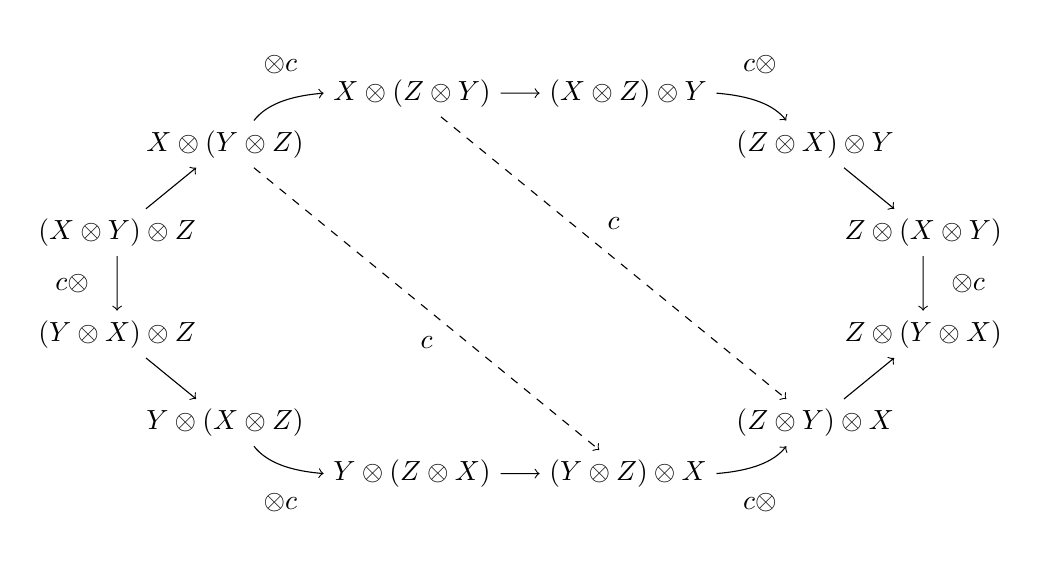
\begin{tikzpicture}[xscale=5.3, yscale=2.5, every edge/.style={draw, ->}, C/.style={inner sep=1em}]
		\node (A1) at (75:1cm) {$(X \otimes Z) \otimes Y$};
		\node (A2) at (105:1cm) {$X \otimes (Z \otimes Y)$};
		\node (A3) at (135:1cm) {$X \otimes (Y \otimes Z)$};
		\node (A4) at (165:1cm) {$(X \otimes Y) \otimes Z$};
		\node (A5) at (195:1cm) {$(Y \otimes X) \otimes Z$};
		\node (A6) at (225:1cm) {$Y \otimes (X \otimes Z)$};
		\node (A7) at (255:1cm) {$Y \otimes (Z \otimes X)$};
		\node (A8) at (285:1cm) {$(Y \otimes Z) \otimes X$};
		\node (A9) at (315:1cm) {$(Z \otimes Y) \otimes X$};
		\node (A10) at (345:1cm) {$Z \otimes (Y \otimes X)$};
		\node (A11) at (15:1cm) {$Z \otimes (X \otimes Y)$};
		\node (A12) at (45:1cm) {$(Z \otimes X) \otimes Y$};

		\draw (A4) edge (A3);	\draw (A3) edge[bend left] node[C, above] {$\identity \otimes c$} (A2); \draw (A2) edge (A1); \draw (A1) edge[bend left] node[C, above] {$c \otimes \identity$} (A12); \draw (A12) edge (A11); \draw (A11) edge node[C, right] {$\identity \otimes c$} (A10);

		\draw (A4) edge node[C, left] {$c \otimes \identity$} (A5); \draw (A5) edge (A6); \draw (A6) edge[bend right] node[C, below] {$\identity \otimes c$} (A7); \draw (A7) edge (A8); \draw (A8) edge[bend right] node[C, below] {$c \otimes \identity$} (A9); \draw (A9) edge (A10);
	
		\draw[dashed] (A3) edge node[C, below] {$c$} (A8);
		\draw[dashed] (A2) edge node[C, above] {$c$} (A9);
	\end{tikzpicture}\end{center}
	其中未标名的箭头都是结合约束, $c$ 代表自明的交换约束.
\end{proposition}
\begin{proof}
	虚线分大图为三块. 左右两块因六角形公理故交换. 中间的四边形因 $c$ 的自然性而交换. 故全图交换.
\end{proof}

\begin{remark}\label{rem:YBE-cat-strict}
	对于 $\mathcal{V}$ 是严格幺半范畴的情形, 上图可以简并到六项, 其交换性无非是说
	\begin{multline*}
		(c(Y,Z) \otimes \identity_X) \, (\identity_Y \otimes c(X, Z)) \, (c(X, Y) \otimes \identity_Z) = \\
		(\identity_Z \otimes c(X, Y)) \, (c(X, Z) \otimes \identity_Y) \, (\identity_X \otimes c(Y, Z)).
	\end{multline*}
	当 $\mathcal{V}$ 是向量空间对张量积构成的辫幺半范畴, 而 $X=Y=Z$ 时, 上式联系于统计物理学中的杨--Baxter 方程 (``杨''代表杨振宁). 习题中将有进一步的阐释.
\end{remark}

\begin{example}\label{eg:braid}\index[sym1]{Braid@$\cate{Braid}$}
	以下将从拓扑视角构造辫范畴 \cate{Braid}.  设 $n \in \Z_{\geq 1}$, 定义
	\[ C_n := \left\{ \text{子集}\; c \subset \R^2: |c|=n \right\}, \]
	或者说是空间 $\left\{ (y_1, \ldots, y_n) \in (\R^2)^n: \text{相异元} \right\}$ 在置换群作用下的商, 它自然地带有拓扑. 今起取定 $p = \{p_1, \ldots, p_n\} \in C_n$. 定义 $n$ 条线的辫子为连续映射 $x: [0,1] \to C_n$ 使得 $x(0) = x(1) = p$ 者. 形象地看, 以时间 $t$ 为纵轴, 则 $x$ 的轨迹给出 $\R^3$ 中 $n$ 条既不自交又不相交, 从 $\{(p_1, 0), \ldots, (p_n, 0) \}$ 上行至 $\{ (p_1, 1), \ldots, (p_n, 1) \}$ 的连续曲线, 是名辫子. 如果辫子 $x_1$ 可以连续变动到 $x_2$, 使得端点 $p$ 全程不变, 则称 $x_1$ 和 $x_2$ 等价. 以下所谓的辫子皆指等价类. 全体 $n$ 条线的辫子所成集合记为 $\mathcal{B}_n$.

	虽然辫子可以视作 $\R^3$ 中的图形, 我们习惯将之压扁到某平面 $L \simeq \R^2$ 上, 过程中可能造成这些曲线的像相交, 但适当扰动 $L$ 可保证任三条曲线的像不共点, 并且无妨假定辫子的头尾两端分别映到 $(i, 0), (i, 1) \in \R^2$, 其中 $i=1, \ldots, n$. 为了保存空间中的信息, 我们在任两条曲线的像的交点标注何者在上, 何者在下. 考虑 $n=3$ 的情形为例:
	\begin{center}\begin{tikzpicture}[baseline=(braid), yscale=0.75]
		\braid[style strands={1}, style strands={2}, style strands={3}] (braid) s_1 s_2^{-1};
		\node[left=1em] (A) at (braid-1-s) {$t=1$};
		\node[left=1em] (B) at (braid-2-e) {$t=0$};
		\draw[-Latex, ultra thick] (B) -- (A);
		\node[below] at (braid-1-e) {$3$};
		\node[below] at (braid-2-e) {$1$};
		\node[below] at (braid-3-e) {$2$};
	\end{tikzpicture} \quad 和 \quad \begin{tikzpicture}[baseline=(braid), yscale=0.75]
		\braid[style strands={1}, style strands={2}, style strands={3}] (braid)  s_2 s_1^{-1};
		\node[below] at (braid-1-e) {$2$};
		\node[below] at (braid-2-e) {$3$};
		\node[below] at (braid-3-e) {$1$};
	\end{tikzpicture}\end{center}

	定义任意 $x, y \in \mathcal{B}_n$ 的合成 $xy$ 为 $x,y: [0,1] \to C_n$ 的首尾相衔; 形象地看, 这无非是粘结 $x$ 的起点与 $y$ 的终端以得到新的辫子. 不难看出这是良定的. 例如上图的两个辫子若依序记作 $x,y$, 则
	\[ xy \; = \;
		\begin{array}{|c|c|} \hline x \\ \hline y \\ \hline \end{array} \quad = \quad
		\begin{tikzpicture}[yscale=0.75, baseline=(braid)]
		\braid[style strands={1}, style strands={2}, style strands={3},
			floor command={
			\draw[dashed] (\floorsx,\floorsy) -- (\floorex,\floorsy);
			}] (braid)
		s_1 s_2^{-1} | s_2 s_1^{-1};
	\end{tikzpicture}\]
	将上图的各条线拉直, 可见它等价于两条垂直线 $\vert\;\vert$. 从代数的视角, $\mathcal{B}_n$ 连同辫子的合成运算构成一个群, 称为 \emph{Artin 辫群}. 乘法结合律是自明的, 乘法幺元是 $\underbracket{\vert \cdots \vert}_{n \text{条}}$, 或者说是常值函数 $[0,1] \to \{p\} \subset C_n$. 而一个辫子 $x$ 的逆元无非是让曲线 $x: [0,1] \to C_n$ 逆行, 或者说是压扁到平面 $\R^2$ 后取其垂直镜像. 熟悉拓扑学的读者当可立刻看出 $\mathcal{B}_n = \pi_1(C_n, p)$; 见例 \ref{eg:fundamental-groupoid}.

	约定 $\mathcal{B}_0$ 为平凡群. 我们将在 \S\ref{sec:symmetric-group} 探究 $\mathcal{B}_n$ 的一些群论性质, 及其与对称群 $\mathfrak{S}_n$ 的联系; 群 $\mathcal{B}_n$ 的一套展示将在 \eqref{eqn:braid-presentation} 给出.\index{bianqun@辫群 (braid group)}\index[sym1]{B_n@$\mathcal{B}_n$}

	现在构造严格幺半范畴 $\cate{Braid}$: 其对象集是 $\Z_{\geq 0}$, 而任两个对象 $n,m$ 间的态射集在 $n=m$ 时定为 $\mathcal{B}_n$, 否则定为空集. 态射的合成即是辫群中的合成. 紧接着定义 $m \otimes n := m+n$, 而对 $x \in \mathcal{B}_m$, $y \in \mathcal{B}_n$, 态射 $x \otimes y \in \mathcal{B}_{m+n}$ 定为两个辫子的并置, 形象地表述为
	\begin{center} 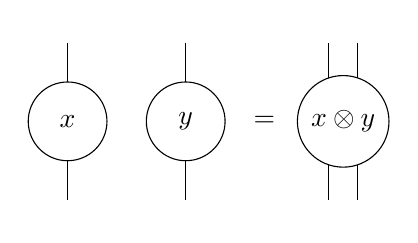
\begin{tikzpicture}[baseline=(current bounding box.center),
		 midbraid/.style={midway, draw, fill=white, shape=circle, minimum size=1cm} ]
		\draw (0,1) -- (0,-1) node[midbraid] {$x$};
		\draw (1.5,1) -- (1.5,-1) node[midbraid] {$y$};
		\node at (2.5,0) {$=$};
		\draw[double distance=10pt] (3.5, 1) -- (3.5,-1) node[midbraid] {$x \otimes y$};
	\end{tikzpicture}\end{center}
	易见 $x \otimes y$ 良定. 并使得 $\cate{Braid}$ 成为严格幺半范畴; 其幺元是 $0$.

	现在定义结合约束 $c$ 以得到辫幺半范畴. 对于 $X=m$, $Y=n$, 我们以
	
\begin{tikzpicture} \draw[black, line width=3pt] (0,0) -- (0.5, 0); \end{tikzpicture}
	表示对应于辫子 $X$ 的 $m$ 条互不缠绕的线, 而以
	
\begin{tikzpicture} \draw[lightgray, line width=3pt] (0,0) -- (0.5, 0); \end{tikzpicture}
	表示对应于辫子 $Y$ 的 $n$ 条互不缠绕的线. 定义 $c(X, Y) \in \mathcal{B}_{m+n}$ 为
	\[ c(m,n) \;= \; \begin{tikzpicture}[baseline=(braid)]
		\braid[style strands={1}{lightgray}, style strands={2}{black}, line width=3pt] (braid) s_1;
		\node[above] at (braid-1-s) {$n$};
		\node[above] at (braid-2-s) {$m$};
		\node[below] at (braid-1-e) {$n$};
		\node[below] at (braid-2-e) {$m$};
	\end{tikzpicture}\]
	这意味着把 $n$ 条线 
\begin{tikzpicture} \draw[lightgray, line width=3pt] (0,0)--(0.5,0); \end{tikzpicture} 视为一个整体, 压过由 
\begin{tikzpicture} \draw[black, line width=3pt] (0,0)--(0.5,0); \end{tikzpicture} 表示的 $m$ 条线. 若再把 $X$ 或 $Y$ 分成两股 $U, V$ 并绘制相应的辫图 (形如
	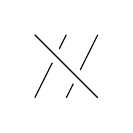
\begin{tikzpicture}[baseline=(current bounding box.center), scale=0.4, wline/.style={color=white, line width=1.8mm}]
		\draw (1,2) -- (0,0);
		\draw (2,2) -- (1,0);
		\draw[wline] (0,2) -- (2,0); \draw (0,2) -- (2,0);
	\end{tikzpicture}
	或
	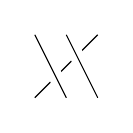
\begin{tikzpicture}[baseline=(current bounding box.center), scale=0.4, wline/.style={color=white, line width=1.8mm}]
		\draw (2,2) -- (0,0);
		\draw[wline] (0,2) -- (1,0); \draw (0,2) -- (1,0);
		\draw[wline] (1,2) -- (2,0); \draw (1,2) -- (2,0);
	\end{tikzpicture} )
	就能验证六角形公理 (注记 \ref{rem:hexagon-axiom-strict}), 细节留给读者.

	杨--Baxter 方程 (注记 \ref{rem:YBE-cat-strict}) 可翻译为一目了然的等式.
	\[ \begin{tikzpicture}[yscale=0.6, baseline=(braid)]
		\braid[style strands={1}, style strands={2}, style strands={3}] (braid) s_1 s_2 s_1;
	\end{tikzpicture}
	\qquad = \qquad
	\begin{tikzpicture}[yscale=0.6, baseline=(braid)]
		\braid[style strands={1}, style strands={2}, style strands={3}] (braid) s_2 s_1 s_2;
	\end{tikzpicture} \]

	同理, 交换约束的自然性直观地诠释如下.
	\begin{center}
	$\begin{tikzcd}
		X \otimes Y \arrow[d, "{f \otimes g}"'] \arrow[r, "{c(X, Y)}"] & Y \otimes X \arrow[d, "{g \otimes f}"] \\
		X \otimes Y \arrow[r, "{c(X, Y)}"'] & Y \otimes X
	\end{tikzcd}$ \quad 交换相当于 \quad
	\begin{tikzpicture}[baseline=(braid),
		midbraid/.style={shape=circle, draw, fill=white, thick, outer sep=0pt, inner sep=0pt, minimum size=5mm} ]
		\coordinate (B1) at (0, 0);
		\coordinate (B2) at (2.2, 0);
		\braid[style strands={1}{lightgray}, style strands={2}{black}, line width=3pt] (bone) at (B1) s_1;
		\node at (bone-1-s) [midbraid, below=3pt] {\small $g$};
		\node at (bone-2-s) [midbraid, below=3pt] {\small $f$};
		\braid[style strands={1}{lightgray}, style strands={2}{black}, line width=3pt] (btwo) at (B2) s_1;
		\node at (btwo-1-e) [midbraid, above=3pt] {\small $g$};
		\node at (btwo-2-e) [midbraid, above=3pt] {\small $f$};
		\node at ($(bone.center)!.5!(btwo.center)$) {$=$};
	\end{tikzpicture}\end{center}
	由于
	\begin{tikzpicture}[baseline=(braid), scale=0.5]
		\braid[style strands={1}{black}, style strands={2}{black}] (braid) s_1;
	\end{tikzpicture} $\neq$
	\begin{tikzpicture}[baseline=(braid), scale=0.5]
		\braid[style strands={1}{black}, style strands={2}{black}] (braid) s_1^{-1};
	\end{tikzpicture},
	幺半范畴 $\cate{Braid}$ 并不对称; 实际上 $c(1, 1)$ 生成无穷循环群群 $\mathcal{B}_2 \simeq \Z$, 这应当是直观的.
\end{example}

我们依靠一些拓扑直觉对 $\cate{Braid}$ 验证了辫结构的各条性质. 反观之, 可以证明 $\cate{Braid}$ 中态射在合成运算下的诸般关系, 亦即辫图的种种等式, 业已囊括一切辫幺半范畴的共性 \cite[Corollary 2.6]{JS93}; 按数学家的``黑话'', $\cate{Braid}$ 乃是``由对象 $1$ 生成的自由辫幺半范畴''. 直白地说, 辫幺半范畴的一般性质可以在 $\cate{Braid}$ 中用直观检验. 相较于定义 \ref{def:braiding} 诸公理, 辫图之间的等式往往是一目了然的, 相信读者在关于杨--Baxter 方程的讨论中已经充分领教过.

\section{充实范畴}\label{sec:enriched-cat}
其实各位已经遇过不少充实范畴. 对充实范畴可以有两种视角:
\begin{compactitem}
	\item 它是范畴论的一种延伸;
	\item 充实范畴是 $\Hom$-集被赋予额外结构的范畴.
\end{compactitem}
前者便于铺陈理论, 也是我们将采用的观点, 而数学家通常倾向于后者. 我们在例 \ref{eg:categories} 中已经看到不少实例, 其中范畴的 $\Hom$ 集经常带有种种额外的结构, 如交换群或拓扑空间等. 充实范畴论的想法是
\begin{center}\begin{tikzpicture}
	\node (A) at (0,0) {$\Hom$-集};
	\node (B) at (4,0) {$\Hom$-对象};
	\node[single arrow, draw] at ($(A)!.5!(B)$) {\footnotesize 代换成};
\end{tikzpicture}\end{center}
然而后者是何种范畴中的对象呢? 我们必须能定义 $\Hom$-对象之间的合成与其中的恒等态射, 幺半范畴为此提供了一套合适的语言. 关于充实范畴的专论可见 \cite{Ke05}.

\begin{definition}\label{def:enriched-cat}\index{chongshifanchou@充实范畴 (enriched category)}
	设 $\mathcal{V}$ 为幺半范畴. 所谓 $\mathcal{V}$-充实范畴或 $\mathcal{V}$-范畴 $\mathcal{C}$, 意谓以下一组资料: \index[sym1]{HomCi@$\iHom_{\mathcal{C}}(X, Y)$}
	\begin{enumerate}
		\item 对象集 $\Obj(\mathcal{C})$;
		\item 对任两个 $X, Y \in \Obj(\mathcal{C})$, 给定态射对象 $\iHom_{\mathcal{C}}(X, Y) \in \Obj(\mathcal{V})$;
		\item 对任三个 $X, Y, Z \in \Obj(\mathcal{C})$, 给定合成态射
			\[ M: \iHom_{\mathcal{C}}(Y, Z) \otimes \iHom_{\mathcal{C}}(X, Y) \longrightarrow \iHom_{\mathcal{C}}(X, Z), \]
			依往例, 我们将经常省略符号 $M$ 并将 $\iHom_{\mathcal{C}}(\cdots)$ 写成 $\iHom(\cdots)$;
		\item 对任意对象 $X \in \Obj(\mathcal{C})$, 给定恒等态射
			\[ \identity_X : \munit \to \iHom_{\mathcal{C}}(X ,X); \]
	\end{enumerate}
	使得以下图表对任意 $X, Y, Z, W \in \Obj(\mathcal{C})$ 皆交换.
	\begin{center} 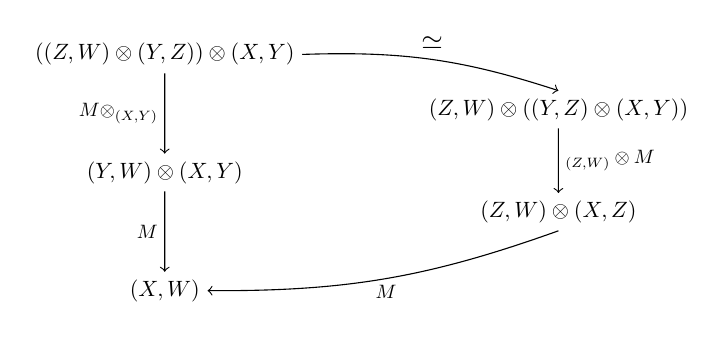
\begin{tikzpicture}[A/.style={scale=0.8, transform shape}, B/.style={scale=0.7, transform shape}, every edge/.style={->, draw}]
		\node[A] (A1) at (0, 3) {$(\iHom(Z, W) \otimes \iHom(Y, Z)) \otimes \iHom(X,Y)$};
		\node[A] (A2) at (0, 1.5) {$\iHom(Y,W) \otimes \iHom(X,Y)$};
		\node[A] (A3) at (0, 0) {$\iHom(X, W)$};
		\node[A] (A4) at (5, 1) {$\iHom(Z,W) \otimes \iHom(X, Z)$};
		\node[A] (A5) at (5, 2.3) {$\iHom(Z,W) \otimes (\iHom(Y,Z) \otimes \iHom(X,Y))$};

		\draw (A1) edge node[B, left] {$M \otimes \identity_{\iHom(X,Y)}$} (A2);
		\draw (A2) edge node[B, left] {$M$} (A3);
		\draw (A4.south) edge[bend left=10] node[B, below] {$M$} (A3.east);
		\draw (A5) edge node[B, right] {$\identity_{\iHom(Z, W)} \otimes M$} (A4);
		\draw (A1.east) edge[bend left=10] node[above]{$\simeq$} (A5.north);
	\end{tikzpicture} \\ \vspace{1.5em}
	\begin{tikzpicture}[A/.style={scale=0.8, transform shape}, B/.style={auto, scale=0.65, transform shape}, every edge/.style={->, draw}]
		\node[A] (T1) {$\iHom(Y, Y) \otimes \iHom(X,Y)$};
		\node[A] (T2) [below=of T1] {$\iHom(X,Y)$};
		\node[A] (T3) [left=of T2] {$\munit \otimes \iHom(X, Y)$};
		\draw (T3.north) edge node[B] {$\identity_Y \otimes \identity_{\iHom(X,Y)}$} (T1.west);
		\draw (T1) edge node[B] {$M$} (T2);
		\draw (T3) edge (T2);
		
		\node[A] (S1) [right=of T1] {$\iHom(X, Y) \otimes \iHom(X,X)$};
		\node[A] (S2) [below=of S1] {$\iHom_{\mathcal{C}}(X,Y)$};
		\node[A] (S3) [right=of S2] {$\iHom(X, Y) \otimes \munit$};
		\draw (S3.north) edge node[B, swap] {$\identity_{\iHom(X,Y)} \otimes \identity_X$} (S1.east);
		\draw (S1) edge node[B, swap] {$M$} (S2);
		\draw (S3) edge (S2);
	\end{tikzpicture} \end{center}
\end{definition}

易见上述交换图表无非是定义 \ref{def:category} 中的态射性质在幺半范畴中的版本. 接着讨论 $\mathcal{V}$-范畴之间的函子. 读者或许已经胸有成竹, 但我们仍不厌其烦地复述如下.

\begin{definition}\label{def:enriched-functor}\index{hanzi!充实情形}
	对于给定之 $\mathcal{V}$-范畴 $\mathcal{C}_1$ 和 $\mathcal{C}_2$, 函子 $F: \mathcal{C}_1 \to \mathcal{C}_2$ 由对象集间的映射 $X \mapsto FX$和 $\Hom$-对象间的态射 $\iHom(X, Y) \to \iHom(FX, FY)$ 给出, 使得以下图表对所有对象 $X, Y, Z$ 交换.
	\[ \begin{tikzcd}
		\iHom(Y, Z) \otimes \iHom(X, Y) \arrow[r] \arrow[d] & \iHom(X, Z) \arrow[d] \\
		\iHom(FY, FZ) \otimes \iHom(FX, FY) \arrow[r] & \iHom(FX, FZ)
	\end{tikzcd} \]
	\[ \begin{tikzcd}
		\iHom(X, X) \arrow[rr] & & \iHom(FX, FX) \\
		& \munit \arrow[lu] \arrow[ru] &
	\end{tikzcd} \]
\end{definition}

\begin{remark}\label{rem:enriched-to-ordinary}
	给定 $\mathcal{V}$-范畴 $\mathcal{C}$, 可以定义一个相应的普通范畴如下: 对象集仍取 $\Obj(\mathcal{C})$, 而态射集取作
	\[ \Hom(X, Y) := \Hom_{\mathcal{V}}\left( \munit, \iHom(X, Y) \right). \]
	恒等态射 $\identity_X: \munit \to \iHom(X, X)$ 因此是 $\Hom(X, X)$ 的元素, 态射的合成定义为
	\[ \begin{tikzcd}
		\Hom_{\mathcal{V}}\left( \munit, \iHom(Y, Z) \right) \otimes \Hom_{\mathcal{V}}\left( \munit, \iHom(X, Y) \right) \arrow[d, "{\otimes \;\text{的函子性}}"] \\
		\Hom_{\mathcal{V}}\left( \munit \otimes \munit, \iHom(Y, Z) \otimes \iHom(X, Y) \right) \arrow[d, "{\text{用 }\; \iota: \munit \otimes \munit \rightiso \munit \text{ 拉回}}"] \\
		\Hom_{\mathcal{V}}\left( \munit, \iHom(X, Z) \right).
	\end{tikzcd} \]
\end{remark}

\begin{definition}\label{def:enriched-naturaltrans}\index{ziranbianhuan!充实情形}
	设 $F, G: \mathcal{C}_1 \to \mathcal{C}_2$ 为 $\mathcal{V}$-范畴间的函子, 自然变换 (或称态射) $\theta: F \to G$ 是一族态射 $\theta_X: \munit \to \iHom(FX, GX)$, 其中 $X$ 取遍 $\Obj(\mathcal{C}_1)$, 使得下图对所有 $X, Y$ 交换.
	\[ \begin{tikzcd}
		\munit \otimes \iHom(X, Y) \arrow[r, "{\theta_Y \otimes F}"] & \iHom(FY, GY) \otimes \iHom(FX, FY) \arrow[d] \\
		\iHom(X, Y) \arrow[u] \arrow[d] & \iHom(FX, GY) \\
		\iHom(X, Y) \otimes \munit \arrow[r, "{G \otimes \theta_X}"'] & \iHom(GX, GY) \otimes \iHom(FX, GX) \arrow[u] .
	\end{tikzcd} \]
\end{definition}
定义之所以这么迂回, 是因为在一般的 $\mathcal{V}$-范畴中无法谈论 $\Hom$-对象里的元素. 自然变换的纵, 横合成的定义留给读者. 由函子与自然变换的充实版本可对 $\mathcal{V}$-范畴定义范畴等价的概念.\index{fanchoudengjia!充实情形}

\begin{example}
	取 $\mathcal{V} = \cate{Set}$, 配上 $\otimes := \times$ 使之成为幺半范畴 (例 \ref{eg:monoidal-cat}), 则 $\mathcal{V}$-范畴无非是之前定义的范畴. 请留意此处仍遵循约定 \ref{con:U-small}, 因此 $\cate{Set}$ 是 $\mathcal{U}$-集构成的范畴, 而范畴意指 $\mathcal{U}$-范畴.
\end{example}

\begin{example}\index{tuopufanchou@拓扑范畴}
	类似地, 取 $\mathcal{V} = \cate{CGHaus}$ (例 \ref{eg:categories}) 及 $\otimes := \times$, 相应的充实范畴称作\emph{拓扑范畴}. 关于使用 $\cate{CGHaus}$ 的缘由可参阅例 \ref{eg:categories} 的讨论, 或参阅 \cite[Chapter 5]{May99}. 
\end{example}

\begin{example}\label{eg:Ab-cat}\index{Ab-fanchou@$\cate{Ab}$-范畴}
	取 $\mathcal{V} := \cate{Ab}$, $\otimes$ 为交换群 (即 $\Z$-模) 的张量积而 $\munit := \Z$, 得到的 $\cate{Ab}$-范畴也称为\emph{预加性范畴}. 其实无需幺半范畴的语言也能定义 $\cate{Ab}$-范畴. 说穿了, $\cate{Ab}$-范畴的特性如下.
	\begin{compactitem}
		\item $\Hom$-集都带有交换群的结构.
		\item 合成映射 $\Hom(Y, Z) \times \Hom(X, Y) \to \Hom(X, Z)$ 是 $\Z$-双线性映射, 即: 满足 $f(g+h) = fg+ fh$, $(g+h)f = gf + hf$. 这是因为根据张量积的性质, 群同态 $\Hom(Y,Z) \dotimes{\Z} \Hom(X, Y) \to \Hom(X, Z)$ 与双线性映射 $\Hom(Y, Z) \times \Hom(X, Y) \to \Hom(X, Z)$ 是一回事.
		\item 展开定义, 可知 $\cate{Ab}$-范畴之间的函子是在 $\Hom$-集间给出群同态的函子.
		\item 对自然变换无额外条件.
	\end{compactitem}
	 凡此种种都符合本节开头提到的视角, 详细验证留作练习. 特别地, 对所有对象 $X, Y$, 在 $\Hom(X, Y)$ 中有良定的零元 $0$, 它与任何可相合成的态射合成后仍是零元. 这是一类极常见的范畴: 举例明之, 任意环 $A$ 上的左模范畴 $A\dcate{Mod}$ 都是 $\cate{Ab}$-范畴, 这也包括了 $\cate{Ab}$ 本身.

	在 $\cate{Ab}$ 的例子中, 由于对任意交换群 $M$ 有自然的双射
	\begin{align*}
		\Hom_{\cate{Ab}}(\Z, M) & \rightiso M \\
		f & \mapsto f(1),
	\end{align*}
	可见函子 $\Hom_{\cate{Ab}}(\munit, \cdot) = \Hom_{\cate{Ab}}(\Z, \cdot): \cate{Ab} \to \cate{Set}$ 同构于忘却函子.  故注记 \ref{rem:enriched-to-ordinary} 的手续施于 $\cate{Ab}$-范畴的效果无非是忘却 $\Hom$-集上的群结构.
\end{example}

由于 $\cate{Ab}$-范畴在数学中经常用到, 我们接着考察它的一些特殊性质. 回顾 \S\ref{sec:limits}. 设 $I$ 为小集合, 则已知在范畴 $A\dcate{Mod}$ 中存在以 $I$ 为指标集的积 $\prod_{i \in I} M_i$ 和余积 $\bigoplus_{i \in I} M_i$ (即模的直和). 当 $I$ 有限时两者相等: 这从 $\prod$ 和 $\bigoplus$ 的具体定义看是一目了然的, 然而这也是 $\cate{Ab}$-范畴共有的普遍现象. 我们引进双积的概念予以解释.

\begin{definition}\label{def:biproduct}\index{shuangji@双积 (biproduct)}
	设 $\mathcal{C}$ 为 $\cate{Ab}$-范畴, $X_1, X_2$ 为其中对象. 则 $X_1, X_2$ 的\emph{双积}意指图表
	\[ \begin{tikzcd}
		X_1 \arrow[r, yshift=-0.5ex, "\iota_1"'] & Z \arrow[l, yshift=0.5ex, "p_1"'] \arrow[r, yshift=0.5ex, "p_2"] & X_2 \arrow[l, yshift=-0.5ex, "\iota_2"]
	\end{tikzcd} \]
	使得 $p_1 \iota_1 = \identity$, $p_2 \iota_2 = \identity$, $\iota_1 p_1 + \iota_2 p_2 = \identity_Z$. 我们也说 $Z$ 连同 $(\iota_1, \iota_2, p_1, p_2)$ 是 $X_1$ 和 $X_2$ 的双积. 记作 $Z = X_1 \oplus X_2$.
\end{definition}
在等式 $\iota_1 p_1 + \iota_2 p_2 = \identity_Z$ 中左合成 $p_2$, 右合成 $\iota_1$, 便得出 $p_2 \iota_1 = 0$; 同理可得 $p_1 \iota_2 = 0$. 双积的构造可以迭代到多变元情形 $Z = X_1 \oplus \cdots \oplus X_n$, 定义条件推广为对 $1 \leq i \leq n$ 给定 $\begin{tikzcd} X_i \arrow[r, yshift=-0.5ex, "\iota_i"'] & Z \arrow[l, yshift=0.5ex, "p_i"'] \end{tikzcd}$, 使得
\begin{gather*}
	p_i \iota_j = \begin{cases} \identity, & i=j \\ 0, & i \neq j \end{cases} \qquad
	\sum_{i=1}^n \iota_i p_i = \identity_Z.
\end{gather*}

\begin{theorem}\label{prop:biproduct-criterion}
	设 $X_1, X_2$ 为 $\cate{Ab}$-范畴 $\mathcal{C}$ 中对象. 以下断言等价
	\begin{compactenum}[(i)]
		\item 积 $X _1\times X_2$ 存在;
		\item 余积 $X_1 \sqcup X_2$ 存在;
		\item $X_1$ 和 $X_2$ 的双积 $Z$存在.
	\end{compactenum}
	若任一断言成立, 则双积 $Z$ 连同 $(p_1, p_2)$ 给出 $X_1$ 和 $X_2$ 的积, 而 $Z$ 连同 $(\iota_1, \iota_2)$ 给出其余积.
\end{theorem}
根据引理 \ref{prop:product-associativity}, 有限积和余积可从二元情形迭代地构造, 这就解释了模的有限直和何以兼具积和余积两种角色.
\begin{proof}
	假设 $X_1, X_2$ 的双积 $Z$ 存在. 由于
	\begin{align*}
		p_1 \iota_2 & = p_1 \circ \identity_Z \circ \iota_2 =  p_1 (\iota_1 p_1 + \iota_2 p_2) \iota_2 = (p_1 \iota_1) p_1 \iota_2 + p_1 \iota_2 (p_2 \iota_2)  \\
		& = p_1 \iota_2 + p_1 \iota_2,
	\end{align*}
	故 $p_1 \iota_2 = 0$. 同理 $p_2 \iota_1 = 0$. 对给定的态射 $X_1 \xleftarrow{f_1} W \xrightarrow{f_2} X_2$, 置 $\phi := \iota_1 f_1 + \iota_2 f_2 : W \to Z$. 由先前公式可导出 $p_i \phi = f_i$ ($i=1,2$). 反之, 若 $\phi: W \to Z$ 满足 $p_i \phi = f_i$, 则
	\[ \phi = (\iota_1 p_1 + \iota_2 p_2) \phi = \iota_1 f_1 + \iota_2 f_2 \]
	唯一确定了 $\varphi$. 因此 $(Z, p_1, p_2)$ 确实满足积的泛性质.

	今假设 $X_1 \xleftarrow{p_1} Z \xrightarrow{p_2} X_2$ 是积. 对于 $i=1,2$, 定义 $\iota_i: X_1 \to Z$ 使得
	\[ \forall j=1,2, \quad  p_j \iota_i =
		\begin{cases}
			\identity_{X_i}, & i=j, \\
			0, & i \neq j .
		\end{cases}
	\]
	仅须验证 $\iota_1 p_1 + \iota_2 p_2 = \identity_Z$ 即可说明 $(Z, \iota_1, \iota_2, p_1, p_2)$ 是双积. 我们有
	\begin{align*}
		p_1 (\iota_1 p_1 + \iota_2 p_2) & = p_1 + 0 = p_1 \circ \identity_Z , \\
		p_2 (\iota_1 p_1 + \iota_2 p_2) & = 0 + p_2 = p_2 \circ \identity_Z.
	\end{align*}
	根据积的泛性质遂有 $\iota_1 p_1 + \iota_2 p_2 = \identity_Z$. 反转箭头便得到余积的情形.
\end{proof}
\begin{remark}
	审视证明可知同构 $\psi: X_1 \sqcup X_2 \rightiso X_1 \times X_2$ 可以取为由
	\[ p_j \psi \iota_i =
		\begin{cases}
			\identity_{X_i}, & i=j, \\
			0, & i \neq j
		\end{cases} \]
	刻画的态射, 其中 $\iota_i : X_i \to X_1 \sqcup X_2$, $p_i: X_1 \times X_2 \to X_i$.
\end{remark}

\begin{lemma}
	设 $X$ 为 $\cate{Ab}$-范畴 $\mathcal{C}$ 中对象. 以下性质等价.
	\begin{compactenum}[(i)]
		\item $X$ 是始对象,
		\item $\identity_X = 0$,
		\item $\End_{\mathcal{C}}(X) = \{0\}$,
		\item $X$ 是终对象.
	\end{compactenum}
	特别地, 如果 $X$ 是始对象或终对象, 则 $X$ 是零对象 (定义 \ref{def:universal-objects}), 而 $0 \in \Hom(X, \cdot)$ 是定义 \ref{def:zero-morphism} 中的零态射.
\end{lemma}
\begin{proof}
	设 $X$ 是 $\mathcal{C}$ 的始对象, 则群 $\End_{\mathcal{C}}(X)$ 仅有一个元素, 它只能是 $0 = \identity_X$, 故 (i) $\implies$ (ii). 由于对每个 $Y$ 和 $f \in \Hom(X, Y)$ 都有 $f \circ \identity_X = f$, 利用 $\cate{Ab}$-范畴的性质可以推出 (ii) $\implies$ (iii) $\implies$ (i). 反转箭头可知 (iv) 与其它条件等价.
\end{proof}

\begin{definition}[加性函子与加性范畴]\label{def:additive-cat}\index{jiaxingfanchou@加性范畴 (additive category)}\index{hanzi!加性情形}
	称 $\cate{Ab}$-范畴之间的函子 (见定义 \ref{def:enriched-functor}) 为\emph{加性函子}. 若 $\cate{Ab}$-范畴 $\mathcal{C}$ 有零对象 $0$, 而且任意 $X, Y \in \Obj(\mathcal{C})$ 有双积 $X \oplus Y$, 则称 $\mathcal{C}$ 为\emph{加性范畴}. 
\end{definition}

先前举出的模范畴 $A\dcate{Mod}$ 是加性范畴的典型例子, 见推论 \ref{prop:Mod-cat-additive}. 函子 $F: \mathcal{C}_1 \to \mathcal{C}_2$ 为加性函子当且仅当 $\Hom_{\mathcal{C}_1}(X, Y) \to \Hom_{\mathcal{C}_2}(FX, FY)$ 对每个 $X, Y$ 都是加法群同态.

\begin{proposition}\label{prop:biproduct-preservation}
	$\cate{Ab}$-范畴之间的加性函子保持双积.
\end{proposition}
\begin{proof}
	若 $F: \mathcal{C} \to \mathcal{C}'$ 是加性函子, 而资料 $(\iota_1, \iota_2, p_1, p_2)$ 定义了 $\mathcal{C}$ 里的双积, 则资料 $(F(\iota_1), F(\iota_2), F(p_1), F(p_2))$ 依然满足双积的条件. 原因在于双积是由等式而非箭头的存在性来定义的.
\end{proof}

\begin{proposition}\label{prop:additive-prod-coprod}
	在加性范畴中任意有限个对象的积和余积存在, 并且两者自然同构.
\end{proposition}
\begin{proof}
	两项的情形无非是关于双积的定理 \ref{prop:biproduct-criterion}, 一般情形则按引理 \ref{prop:product-associativity} 的结合约束化到两项.
\end{proof}

\section{\texorpdfstring{$2$}{2}-范畴一瞥}\label{sec:2-cat}
我们已经习惯将范畴的对象表示为点, 而将态射表示为其间的箭头; 这种图示中维度最高的构造是一维的箭头, 所以不妨称范畴为 $1$-范畴. 忘掉箭头的范畴无非是集合, 剩下的仅有零维的对象, 所以集合可以设想为 $0$-范畴. 于是引出一个自然的问题: 如何定义高阶范畴? 本节仅探讨 $2$ 阶的情形, 换言之, 我们要在点与箭头之外添上某些 $2$ 维构造, 称为 $2$-胞腔.

$2$-范畴并非无端的空想, 譬如例 \ref{eg:Cat} 考虑的 $\cate{Cat}$ 就是一个标准例子; 另一个自然的例子是考虑拓扑空间 (点), 其间的连续映射 (箭头), 与映射之间的同伦 ($2$-胞腔). 尽管想法简单, 如何萃取合适的定义却是一大问题. 以下定义的版本又称严格 $2$-范畴.

\begin{definition}\index{$2$-范畴}
	一个 (严格) $2$-范畴 $\mathcal{C}$ 意指以下资料
	\begin{itemize}
		\item 对象, 或称 $0$-态射构成的集合 $\Obj(\mathcal{C}) = \Mor_0(\mathcal{C})$;
		\item $1$-态射构成的集合 $\Mor_1(\mathcal{C}) = \bigsqcup_{X, Y \in \Mor_0(\mathcal{C})} \Hom(X, Y)$;
		\item $2$-态射构成的集合 $\Mor_2(\mathcal{C}) = \bigsqcup_{a, b \in \Mor_1(\mathcal{C})} \Hom(a, b)$.
	\end{itemize}
	习惯将 $1$-态射写成 $f: X \to Y$, 而 $2$-态射写成 $\theta: a \Rightarrow b$ 的形式. $\mathcal{C}$ 中有以下几种运算.
	\begin{enumerate}[(i)]
		\item 我们要求 $\mathcal{C}$ 的对象连同 $1$-态射构成一个 ($1$-)范畴.
		% $1$-态射的合成 $\Hom(Y, Z) \times \Hom(X, Y) \to \Hom(X, Z)$, 其中 $X, Y, Z$ 是对象; 这里要求合成运算满足结合律, 并且对每个对象 $X$ 存在幺元 $\identity_X$. 换言之, 我们要求 $\mathcal{C}$ 的对象和 $1$-态射构成一个范畴.
		\item $2$-态射有纵, 横两种合成. 先看纵合成: 令 $X, Y$ 为对象, $f, g, h: X \to Y$ 为 $1$-态射, $\theta: f \Rightarrow g$, $\psi: g \Rightarrow h$ 为 $2$-态射, 则有纵合成 $\psi \circ \theta: f \Rightarrow h$, 图示为
			\[ \begin{tikzcd}
				X
				\arrow[bend left=60, rr, "f", ""' name=U]
				\arrow[rr, "g"' name=M, "" name=MM]
				\arrow[bend right=60, rr, "" name=D, "h"'] & &
				\arrow[Rightarrow, to path=(U) -- (MM) \tikztonodes, "\theta"] \arrow[Rightarrow, to path=  (M) -- (D) \tikztonodes, "\psi"]  Y
			\end{tikzcd}
			\quad \text{合成为} \quad
			\begin{tikzcd}
				X
				\arrow[bend left=50, rr, "f", ""' name=U]
				\arrow[bend right=50, rr, "" name=D, "h"']
				& & \arrow[Rightarrow, to path=(U) -- (D) \tikztonodes, "\psi \circ \theta"] Y .
			\end{tikzcd} \]
		\item 接着看横合成. 令 $X, Y ,Z$ 为对象, \begin{tikzcd} X \arrow[r, bend left=20, "f"] \arrow[r, bend right=20, "g"'] & Y \end{tikzcd}, \begin{tikzcd} Y \arrow[r, bend left=20, "f'"] \arrow[r, bend right=20, "g'"'] & Z \end{tikzcd} 为两对 $1$-态射, 而 $\theta: f \Rightarrow g$ 和 $\psi: f' \Rightarrow g'$ 为 $2$-态射, 则有横合成 $\psi \circ \theta: f'f \Rightarrow g'g$, 图示为
			\[ \begin{tikzcd}
				X \arrow[bend left=50, r, "f", ""' name=LU] \arrow[bend right=50, r, "" name=LD, "g"'] &
				Y \arrow[bend left=50, r, "f'", ""' name=RU] \arrow[bend right=50, r, "" name=RD, "{g'}"'] &
				\arrow[Rightarrow, to path=(LU) -- (LD) \tikztonodes, "\theta"] \arrow[Rightarrow, to path=(RU) -- (RD) \tikztonodes, "\psi"] Z
			\end{tikzcd}
			\quad \text{合成为} \quad
			\begin{tikzcd}
				X
				\arrow[bend left=40]{rr}{f'f}[name=U, below]{}
				\arrow[bend right=40]{rr}[name=D]{}[below]{g'g}
				& & \arrow[Rightarrow, to path=(U) -- (D) \tikztonodes]{}{\psi \circ \theta} Z .
			\end{tikzcd} \]
	\item 形如
		\begin{tikzcd}
			X
			\arrow[bend left=30]{rr}{f}[name=U, below]{}
			\arrow[bend right=30]{rr}[name=D]{}[below]{g}
			& & \arrow[Rightarrow, to path=(U) -- (D) \tikztonodes]{}{\theta} Y
		\end{tikzcd}
		的图表称作 $2$-胞腔. 我们要求横合成满足严格的结合律 $\phi \circ (\psi \circ \theta) = (\phi \circ \psi) \circ \theta$, 并且对每个对象 $X$ 都有横幺元 (或者该叫横幺胞腔) $\identity_{X, 2}: \identity_X \Rightarrow \identity_X$, 使得 $\theta \circ \identity_{X, 2} = \theta$, $\identity_{X, 2} \circ \psi = \psi$, 只要上述横合成有意义.
	\item 同样地, 要求 $2$-胞腔的纵合成满足严格结合律, 并且对每个 $1$-态射 $f$ 都有纵幺元 $\identity_f: f \Rightarrow f$.
	\item 纵幺元的横合成仍为纵幺元:
		\[ \begin{tikzcd}
		X \arrow[bend left=50, r, "f", ""' name=LU] \arrow[bend right=50, r, "" name=LD, "f"'] &
		Y \arrow[bend left=50, r, "{f'}", ""' name=RU] \arrow[bend right=50, r, "" name=RD, "{f'}"'] &
		\arrow[Rightarrow, to path=(LU) -- (LD) \tikztonodes, "{\identity_f}"] \arrow[Rightarrow, to path=(RU) -- (RD) \tikztonodes, "{\identity_{f'}}"]  Z
	\end{tikzcd}
	\quad \text{横合成为} \quad
	\begin{tikzcd}
		X
		\arrow[bend left=40, rr, "{f'f}", ""' name=U]
		\arrow[bend right=40, rr, "{f'f}"', "" name=D]
		& & \arrow[Rightarrow, to path=(U) -- (D) \tikztonodes, "{\identity_{f'f}}"] Z .
	\end{tikzcd} \]
	\item 纵横合成之间满足互换律: 对于图表
		\[ \begin{tikzcd}
			X
			\arrow[bend left=60, rr, ""' name=U]
			\arrow[rr, "" name=MM, ""' name=M]
			\arrow[bend right=60, rr, "" name=D] & &
			\arrow[Rightarrow, to path=(U) -- (MM) \tikztonodes, "\theta"] \arrow[Rightarrow, to path=  (M) -- (D) \tikztonodes, "\psi"] Y
			\arrow[bend left=60, rr, ""' name=V]
			\arrow[rr, "" name=NN, ""' name=N]
			\arrow[bend right=60, rr, "" name=E] & &
			\arrow[Rightarrow, to path=(V) -- (NN) \tikztonodes, "\theta'"] \arrow[Rightarrow, to path=  (N) -- (E) \tikztonodes, "\psi'"] Z
		\end{tikzcd} \]
		我们有
		\[ \left( \psi' \underset{\text{纵}}{\circ} \theta'\right) \underset{\text{横}}{\circ} \left( \psi \underset{\text{纵}}{\circ} \theta\right) = \left( \psi' \underset{\text{横}}{\circ} \psi \right) \underset{\text{纵}}{\circ} \left( \theta' \underset{\text{横}}{\circ} \theta\right).  \]
	\end{enumerate}
\end{definition}

\begin{remark}
	这里的定义显然违背了注记 \ref{rem:strict-or-not} 的精神, 因为我们要求态射合成满足严格的结合律与幺元性质. 对于 $2$-范畴, 有些定义较为宽松, 同时也远为复杂的版本, 例如所谓的双范畴; 幸运的是双范畴也满足融贯定理, 也就是说任意双范畴皆等价于某个 $2$-范畴 (请对照幺半范畴的定义及其融贯定理 \ref{prop:ML-coherence}). 这般的融贯现象对超过 $2$ 阶的范畴不再成立. 篇幅所限, 就此打住.
\end{remark}

\begin{example}\label{eg:Cat}\index[sym1]{Cat@$\cate{Cat}$}
	$2$-范畴的典型例子是 $\cate{Cat}$, 不妨先粗略地设想为``范畴的范畴'', 这般朴素的想象很快会撞上集合论的困难. 在此我们必须选定一个 Grothendieck 宇宙 $\mathcal{U}$, 依约定 \ref{con:U-small} 区分范畴与小范畴. 现在可以定义 $2$-范畴 $\cate{Cat}$ 如下.
	\begin{compactitem}
		\item 对象或 $0$-态射: 所有小范畴构成的集合,
		\item $1$-态射: $\Hom(\mathcal{C}_1, \mathcal{C}_2)$ 定义为从 $\mathcal{C}_1$ 到 $\mathcal{C}_2$ 的函子所成集合.
		\item $2$-态射: $\Hom(\alpha, \beta)$ 定义为自然变换 $\theta: \alpha \to \beta$ 所成的集合.
		\item $1$-态射的合成定为函子合成; $2$-态射的纵, 横两种合成各自定为自然变换的纵, 横合成.
	\end{compactitem}
	纵横幺元的定义是显然的, 不必多说. 引理 \ref{prop:naturaltrans-associativity} 确保 $\cate{Cat}$ 满足 $2$-范畴的公理.
\end{example}

若忘掉 $\cate{Cat}$ 的 $2$-态射, 只看其普通的范畴结构, 则 $\cate{Cat}$ 带有自然的幺半结构: 其中的运算 $\otimes$ 取为范畴的积 $\times$, 而幺元 $\munit$ 是仅有一个态射的范畴 (回忆例 \ref{eg:categories}). 注意到 $\times$ 可以理解为范畴 $\cate{Cat}$ 中的积, 而 $\munit$ 是 $\cate{Cat}$ 的终对象, 因此这里的构造是例 \ref{eg:monoidal-cat} 的一个特殊情形.

\begin{remark}
	现在可以用充实范畴的想法理解 $2$-范畴. 设 $\mathcal{C}$ 为 $2$-范畴. 对其任意对象 $X, Y$, 定义纵范畴 $\mathcal{V}(X, Y)$ 使得其对象为 $1$-态射 $f: X \to Y$ 而其态射为 $2$-态射 $\theta: f \Rightarrow g$, 态射的合成由 $2$-态射的纵合成给出. 纵结合律和纵幺元 $\identity_f: f \Rightarrow f$ 的性质确保 $\mathcal{V}(X, Y)$ 确实是范畴. 以下假设每个 $\mathcal{V}(X, Y)$ 皆是小范畴. 对于 $\cate{Cat}$, 相应的纵范畴 $\mathcal{V}(\mathcal{C}_1, \mathcal{C}_2)$ 无非是 \S\ref{sec:functor-category} 所定义的函子范畴 $\text{Fct}(\mathcal{C}_1, \mathcal{C}_2)$.

	重述 $2$-范畴 $\mathcal{C}$ 的结构如下:
	\begin{compactitem}
		\item 对象集 $\Obj(\mathcal{C})$;
		\item 对任意 $X, Y \in \Obj(\mathcal{C})$, 指定一个范畴 $\mathcal{V}(X, Y)$;
		\item 对任意 $X, Y, Z \in \Obj(\mathcal{C})$, 指定二元函子
			\[ \circ: \mathcal{V}(Y, Z) \times \mathcal{V}(X, Y) \to \mathcal{V}(X, Z); \]
		\item 对任意 $X \in \Obj(\mathcal{C})$, 指定函子
			\[ U_X: \munit \to \mathcal{V}(X, X); \]
		\item 我们要求函子 $\circ$ 满足严格的结合律, 而 $U_X$ 对 $\circ$ 满足幺元的性质.
	\end{compactitem}
	实际上, 函子 $\circ: \mathcal{V}(Y, Z) \times \mathcal{V}(X, Y) \to \mathcal{V}(X, Z)$ 在其对象层面蕴藏了 $1$-态射的合成运算, 在其态射层面蕴藏了 $2$-态射的横合成运算, 可以验证它同时还蕴涵横幺元的性质与 $2$-范畴定义中的互换律. 选取函子 $U_X: \munit \to \mathcal{V}(X, X)$ 相当于在 $\Hom(X, X)$ 中标出一个对象, 这正是 $\identity_X$.

	综之, $2$-范畴无非是由 $\cate{Cat}$-充实的范畴: 对于任意对象 $X, Y \in \Obj(\mathcal{C})$, 我们把 $\Hom$-集 $\Hom(X, Y)$ 充实为纵范畴 $\iHom(X, Y) := \mathcal{V}(X, Y)$, 后者是幺半范畴 $\cate{Cat}$ 的对象, 如此一来就接上了充实范畴的定义 \ref{def:enriched-cat}.
\end{remark}

\begin{definition}
	$2$-范畴之间的 $2$-函子与 $2$-自然变换按照 $\cate{Cat}$-充实范畴的方法定义 (参看定义 \ref{def:enriched-functor}, \ref{def:enriched-naturaltrans}).
\end{definition}
读者不妨试着写开这些定义. 例如 $2$-函子的定义是将 $i$-态射映到 $i$-态射 (此处 $i=0,1,2$), 并保持这些态射的来源/目标, 合成与幺元等诸般性质.

\begin{convention}
	我们对 $2$-范畴沿用处理自然变换 (即 $2$-范畴 $\cate{Cat}$) 时引入的一些图表, 例如 \S\ref{sec:functors} 中形如
	\[ \begin{tikzcd}
		X \arrow[r, "h"] & Y \arrow[bend left=50, r, "f", ""' name=U] \arrow[bend right=50, r, "" name=D, "g"'] & Z \arrow[Rightarrow, to path=(U)--(D) \tikztonodes, "\theta"] \arrow[r, "k"] & W
	\end{tikzcd} \]
	的横合成, 其确切含义是将 $1$-态射 $h, k$ 各自``拉开''成 $2$-胞腔 $\identity_h, \identity_k$, 再进行横合成. 同理, 注记 \ref{rem:triangle-identity} 中引入的图表
	\[\begin{tikzcd}
		{} & X \arrow[rr, "\identity", ""' name=I] \arrow[rd, "f"] \arrow[Rightarrow, d, "\varepsilon"] & & X \\
		Y \arrow[ru, "g"] \arrow[rr, "" name=J, "\identity"'] & {} & Y \arrow[ru, "g"'] \arrow[Leftarrow, to path= -- (I) \tikztonodes, "\eta"] &
	\end{tikzcd} \]
	代表 $2$-范畴中的合成
	\[ \begin{tikzcd}
		Y \arrow[r, "g"] \arrow[bend right=60, rr, "" name=J, "\identity"'] &
		X \arrow[r, "f"] \arrow[bend left=60, rr, "\identity", ""' name=I] \arrow[Rightarrow, to path= --(J) \tikztonodes, "\varepsilon"] &
		Y \arrow[r, "g"] \arrow[Leftarrow, to path= -- (I) \tikztonodes, "\eta"] &
		X .
	\end{tikzcd} \]
\end{convention}

\begin{remark}\index{bansuidui}
	在 \S\ref{sec:adjoint-functor} 探讨的伴随对 $(F, G, \eta, \varepsilon)$ 可以用 $2$-范畴的语言改写. 设
	\[\begin{tikzcd}
		X \arrow[yshift=0.5ex, r, "f"] & Y \arrow[yshift=-0.5ex, l, "g"]
	\end{tikzcd}\]
	为 $2$-范畴 $\mathcal{C}$ 中的一对 $1$-态射, 而 $\eta: \identity_X \Rightarrow gf$ 和 $\varepsilon: fg \Rightarrow \identity_Y$ 是 $2$-态射. 若它们满足注记 \ref{rem:triangle-identity} 中的三角等式, 则称 $(f, g, \eta, \varepsilon)$ 是伴随对. 取 $\mathcal{C} = \cate{Cat}$ 就回到伴随对的经典定义. 伴随函子的许多性质可以推广到 $2$-范畴情形, 例如伴随等价定理 \ref{prop:adjoint-equivalence} 的证明就完全可以照搬.
\end{remark}

\begin{Exercises}
	\item 对于一般幺半范畴中的对象 $X_1, \ldots, X_n$, 有种种方式能构作它们的 $n$-重 $\otimes$ 运算, 取决于安插括号的方法, 如 $\cdots \otimes (X_i \otimes X_{i+1}) \cdots$ 等等. 证明括号的放法恰有 $\frac{1}{n+1} \binom{2n}{n}$ 种. \begin{hint} 此即组合学中的 Catalan 数. \end{hint}
	\item 证明对任意幺半范畴, $\End(\munit)$ 对态射的合成交换. \begin{hint} 应用引理 \ref{prop:Kelly} 和 $(f \otimes \identity)(\identity \otimes g) = f \otimes g = (\identity \otimes g) (f \otimes \identity)$.\end{hint}
	\item 考虑全体有限全序集和保序映射所成范畴 $\cate{On}_f$. 对于有限全序集 $\sigma$, $\tau$, 在 $\sigma \sqcup \tau$ 上定义唯一的全序使得 $\sigma$ 和 $\tau$ 到 $\sigma \sqcup \tau$ 的嵌入是保序的, 而且 $\sigma$ 中的元素总小于 $\tau$ 中元素. 证明 $\sqcup$ 赋予 $\cate{On}_f$ 自然的幺半范畴结构, 其幺元是空集.
	\item 承上, 说明存在唯一的同构 $c(\sigma, \tau): \sigma \sqcup \tau \rightiso \tau \sqcup \sigma$, 证明 $(\cate{On}_f, \sqcup, c)$ 构成对称幺半范畴.
	\item 本题假定读者熟悉向量空间的张量积. 令 $V$ 为域 $\Bbbk$ 上的向量空间, $R$ 为 $V \otimes V$ 的线性自同构, 相应的杨--Baxter 方程定义作
		\[ (R \otimes \identity_V) \, (\identity_V \otimes R) \, (R \otimes \identity_V) = (\identity_V \otimes R) \, (R \otimes \identity_V) \, (\identity_V \otimes R) , \]
		其中每一项都是 $V \otimes V \otimes V$ 的线性自同构. 设 $\{e_i\}_{i \in I}$ 是 $V$ 的基, 将 $R$ 按 $R(e_i \otimes e_j) = \sum_{k,l} R^{k,l}_{i,j} e_k \otimes e_l$ 展开, 那么上述方程化作
		\[ \forall i,j,k,l,m,n, \quad \sum_{p,q,y} R^{p,q}_{i,j} R^{y,n}_{q,k} R^{l,m}_{p,y} = \sum_{y,q,r} R^{q,r}_{j,k} R^{l,y}_{i,q} R^{m,n}_{y,r}.  \]
		显然此方程不易求解. 如果 $\mathcal{V}$ 是 $(\cate{Vect}(\Bbbk), \otimes, \ldots)$ 的一个幺半子范畴, 且具有辫结构 $c$, 那么对任意 $V \in \Obj(\mathcal{V})$, 从 $R := c(V,V)$ 可得出杨--Baxter 方程的解. 这些方程和一些量子可积系统密切相关. 这也解释了命题 \ref{prop:YBE-cat-strict} 的背景. 请验证上述论断.
		
		现在引进参数 $q \in \Bbbk^\times$. 对于有限维 $\Bbbk$-向量空间 $V = \bigoplus_{i=1}^h \Bbbk e_i$, 证明
		\[ R(e_i \otimes e_j) = \begin{cases}
			e_j \otimes e_i, & i < j, \\
			q e_i \otimes e_j, & i = j, \\
			e_j \otimes e_i + (q - q^{-1}) e_i \otimes e_j, & i > j
		\end{cases} \]
		给出杨--Baxter 方程的解, 并且满足 $\left( R - q \cdot \identity_{V \otimes V} \right) \left( R + q^{-1} \cdot \identity_{V \otimes V} \right) = 0$. 当 $q=1$ 时它退化为 $\cate{Vect}(\Bbbk)$ 上标准的辫结构 $v \otimes w \mapsto w \otimes v$. \index{YBE}

	\item 设 $(\mathcal{V}, \otimes, \ldots)$ 为幺半范畴. 为简便起见, 以下设其为严格幺半范畴, 省略结合约束等态射和括号. 定义幺半范畴 $Z(\mathcal{V})$ 使得:
		\begin{itemize}
			\item 其对象为 $(X, \Phi)$, 其中 $X$ 是 $\mathcal{V}$ 的对象而 $\Phi: (X \otimes -) \rightiso (- \otimes X)$ 是函子的同构, 我们进一步要求对所有对象 $Y,Z$, 下图交换.
				\[\begin{tikzcd}[column sep=small]
					X \otimes Y \otimes Z \arrow[rr, "\Phi_{Y \otimes Z}"] \arrow[rd, "{\Phi_Y \otimes \identity_Z}"'] & & Y \otimes Z \otimes X \\
					&  Y \otimes X \otimes Z \arrow[ru, "{\identity_Y \otimes \Phi_Z}"'] &
				\end{tikzcd}\]
			\item 从 $(X, \Phi)$ 到 $(Y, \Psi)$ 的态射取为所有满足下式的 $f \in \Hom_{\mathcal{V}}(X,Y)$
				\[ \forall Z \in \Obj(\mathcal{V}),\quad (\identity_Z \otimes f) \Phi_Z = \Psi_Z (f \otimes \identity_Z) \; \in \Hom_{\mathcal{V}}(X \otimes Z, Z \otimes Y); \]
			\item 取 $(X, \Phi) \otimes (Y, \Psi)$ 为 $(X \otimes Y,\; (\Phi \otimes \identity)(\identity \otimes \Psi))$. 定义 $Z(\mathcal{V})$ 之幺元为 $\left(\munit, (\identity_X)_{X \in \Obj(\mathcal{V})}\right)$.
		\end{itemize}
		验证这确实给出幺半范畴. 此外 $Z(\mathcal{V})$ 具有自然的辫结构, 试阐明之. 范畴 $Z(\mathcal{V})$ 称为 $\mathcal{V}$ 的 Drinfeld 中心, 这是幺半群中心的一种范畴化.
	\item 验证例 \ref{eg:Ab-cat} 中 $\cate{Ab}$-范畴的刻画确实符合充实范畴的一般理论.
	\item 对给定的函子 $\mathcal{A} \xrightarrow{S} \mathcal{C} \xleftarrow{T} \mathcal{B}$, 按定义 \ref{def:comma-category} 构造范畴 $(S/T)$ (回忆其对象形如 $(A,B,f)$) 及投影函子 $P,Q$. 定义态射 $\alpha: SP \to TQ$ 为 $SP(A,B,f) = \left[ SA \xrightarrow{f} TB \right] = TQ(A,B,f)$. 证明 $\alpha$ 确实是函子间的态射, 而且
		\[\begin{tikzcd}
			(S/T) \arrow[r, "P"] \arrow[d, "Q"'] & \mathcal{A} \arrow[d, "S"] \arrow[Rightarrow, ld, "\alpha" description] \\
			\mathcal{B} \arrow[r, "T"'] & \mathcal{C}
		\end{tikzcd}\]
		是 $2$-范畴 $\cate{Cat}$ 中的 $2$-胞腔.
\end{Exercises}
